


\newpage


\section{Exploration of an Interdisciplinary Scientific Landscape}{Exploration d'un paysage scientifique interdisciplinaire}

\label{app:sec:cybergeo}


%----------------------------------------------------------------------------------------






%----------------------------------------------------------------------------------------

Patterns of interdisciplinarity in science can be quantified through diverse complementary dimensions. This paper studies as a case study the scientific environment of a generalist journal in Geography, \emph{Cybergeo}, in order to introduce a novel methodology combining citation network analysis and semantic analysis. We collect a large corpus of around 200,000 articles with their abstracts and the corresponding citation network that provides a first citation classification. Relevant keywords are extracted for each article through text-mining, allowing us to construct a semantic classification. We study the qualitative patterns of relations between endogenous disciplines within each classification, and finally show the complementarity of classifications and of their associated interdisciplinarity measures. The tools we develop accordingly are open and reusable for similar large scale studies of scientific environments.
\keywords{Citation Network \and Semantic Network \and Interdisciplinarity \and Geography}
% \PACS{PACS code1 \and PACS code2 \and more}
% \subclass{MSC code1 \and MSC code2 \and more}
\end{abstract}

%%%%%%%%%%%%%%%%%%%%%%%
\section*{Introduction}
\label{sec:intro}
%%%%%%%%%%%%%%%%%%%%%%%


The development of interdisciplinary approaches is increasingly necessary for most of disciplines, both for further knowledge discovery but also societal impact of discoveries, as it was recently coined by the special issue of Nature~\citep{natureInterdisc}. \cite{banos2013pour} suggests that the development of such approaches must occur within a subtle spiral between and inside disciplines. An other way to understand this phenomenon is to understand it as the emergence of vertically integrated fields conjointly with horizontal questions as detailed in the Complex Systems roadmap (\cite{2009arXiv0907.2221B}). There are naturally multiple views on what is exactly interdisciplinarity (many other terms such as trans-disciplinarity, cross-disciplinarity also exist) and it actually depends on involved domains : recent hybrid disciplines (see e.g. the ones underlined  by \cite{bais2010praise} such as astro-biology) are a good illustration of the case where entanglement is strong and new discoveries are vertically deep, whereas more loose fields such as ``urbanism'', which have no precise definition and where integration is by essence horizontal, are an other illustration of how transversal knowledge can be produced. Interaction between disciplines are not always smooth, as shows the misunderstandings when urban issues were recently introduced to physicists as \cite{dupuy2015sciences} recalls.


These concerns are part of an understanding of processes of knowledge production, i.e. the \emph{Knowledge of the knowledge} as \cite{morin1986methode} puts it, in which evidence-based perspectives, involving quantitative approaches, play an important role. These paradigms can be understood as a \emph{quantitative epistemology}. Quantitative measures of interdisciplinarity would therefore be part of a multidimensional approach of the study of science that is in a way ``beyond bibliometrics''~\citep{cronin2014beyond}. The focus of this paper is positioned within this stream of research. We first review existing approaches to the measure of interdisciplinarity.


The possible methods for quantitative insights into epistemology are numerous. A good illustration of the variety of approaches is given by network analysis Using citation network features, a good predicting power for citation patterns is for example obtained by~\cite{2013arXiv1310.8220N}. Co-authorship networks can also be used for predictive models~\citep{2014arXiv1402.7268S}. A multilayer network approach was proposed in~\cite{omodei2017evaluating}, using bipartites networks of papers and scholars, in order to produce measures of interdisciplinarity using generalized centrality measures. Disciplines can be stratified into layers to reveal communities between them and therein collaboration patterns~\citep{2015arXiv150601280B}. Keyword networks are used in other fields such as economics of innovation: for example, \cite{choi2014patent} proposes a method to identify technological opportunities by detecting important keywords from the point of view of topological measures. In a similar manner, \cite{shibata2008detecting} uses topological analysis of the citation network to detect emerging research fronts.



Definitions of interdisciplinarity itself and indicators to measure it have already been tackled by a large body of literature. \cite{huutoniemi2010analyzing} recall the difference between \emph{multidisciplinary} (an aggregate of works from different disciplines) and \emph{interdisciplinary} (implying a certain level of integration) approaches. They construct a qualitative framework to classify types of interdisciplinarity, and for example distinguish empirical, theoretical and methodological interdisciplinarities. The multidimensionnal aspect of interdisciplinarity is confirmed even within a specific field such as literature~\citep{austin1996defining}. A first way to quantify interdisciplinarity of a set of publications is to look at the proportion of disciplines outside a main discipline in which they are published, as~\cite{rinia2002impact} do for the evaluation of projects in physics, complementary with judgement of experts. \cite{porter2007measuring} designate this measure as \emph{specialization}, and compares it with a measure of \emph{integration}, given by the spread of citations  done by a paper within the different Subject Categories (classification of the Web of Knowledge), which is also called the \emph{Rao-Stirling} index. \cite{lariviere2010relationship} uses it on a Web of Science corpus to show the existence of an optimal intermediate level of interdisciplinarity for the citation impact within a five year window. A similar work is done in~\citep{lariviere201410}, focusing on the evolution of measures on a long time range. The influence of missing data on this index is studied by \cite{moreno2016uncertainty}, providing an extended framework taking into account uncertainty. The use of networks has also been proposed : \cite{porter2009science} combine the integration index with a mapping technique which consists in visualisation of synthetic networks constructed by co-citations between disciplines. \cite{leydesdorff2007betweenness} shows that the betweenness centrality is a relevant indicator of interdisciplinarity, when considering appropriate citation neighborhood.



We develop in this paper a case study coupling citation network exploration and analysis with text-mining, aiming at mapping the scientific landscape in the neighborhood of a particular journal. We choose to study an electronic journal in Geography, named \textit{Cybergeo}\footnote{\texttt{http://cybergeo.revues.org/}}, that publishes articles within all subfields of Geography and is in that way multidisciplinary. The choice is initially due to data availability, but ensures several constraints making it highly relevant to the context given above. First of all, the ``discipline'' of Geography is very broad and by essence interdisciplinary~\cite{bracken2016interdisciplinarity} : the spectrum ranges from Human and Critical geography to physical geography and geomorphology, and interactions between these subfields are numerous. Secondly, bibliographical data is difficult to obtain, raising the concern of how the perception of a scientific landscape may be shaped by actors of the dissemination and thus far from objective, and making technical solutions as the ones we will consequently develop here crucial tools for an open and neutral science. Finally it makes a particularly interesting case study as the editorial policy is generalist and concerned with open science issues such as peer-review ethics transparency~\citep{10.1371/journal.pone.0147913}, open data and model practices, as recalled by~\cite{pumain2015adapting}, and this work contributes to these by fostering the opening of reflexivity.


Our approach combine semantic communities analysis with citation network to extract features such as interdisciplinarity measures. Our contribution differs from the previous works quantifying interdisciplinarity as it does not assume predefined domains nor classification of the considered papers, but reconstructs from the bottom-up the fields with the endogenous semantic information. \cite{nichols2014topic} already introduced a close approach, using Latent Dirichlet Allocation topic modeling to characterize interdisciplinarity of awards in particular sciences. \cite{palchykov2016ground} takes a similar approach for papers in physics based on concept extraction from full texts, and show that the endogenous classes differ from the top-down subjects classification. Semantic networks are otherwise well studied in social sciences, such as for example \cite{2015arXiv151003797G} that analyze semantic networks of political debates.


Our contribution is original and significant on at least two aspects :
\begin{enumerate}
	\item we combine endogenous classifications in a network multilayer fashion, using semantic information ;
	\item a large dataset is constructed from scratch to study a journal not referenced in main databases, tackling both data retrieval and large scale data processing issues.
\end{enumerate}



The rest of the paper is organized as follows : we describe in the next section the dataset used and the data collection procedure. We then study properties of the citation network and describe the procedure to construct the semantic classification through text-mining. We finally study complementary measures of interdisciplinarity obtained with the different classifications.




%%%%%%%%%%%%%%%%%%%%%%%
\section*{Database Construction}
\label{sec:data}
%%%%%%%%%%%%%%%%%%%%%%%



Our approach imposes some requirements on the dataset used, namely: (i) cover a certain neighborhood of the studied journal in the citation network in order to have a consistent view on the scientific landscape; (ii) have at least a textual description for each node. For these to be met, we need to gather and compile data from heterogeneous sources. We use therefore an application specifically designed, which general architecture is given in Fig.~\ref{fig:datacollection}. Source code of the application and all scripts used in this paper are available on the open \texttt{git} repository of the project\footnote{at \texttt{https://github.com/JusteRaimbault/HyperNetwork}}. Raw and processed data are also openly available on Dataverse\footnote{at \texttt{http://dx.doi.org/10.7910/DVN/VU2XKT}}. We recall that an important contribution of this paper is the construction of such an hybrid dataset from heterogeneous sources, and the development of associated tools that can be reused and further developed for similar purposes.



%%%%%%%%%%%%%%%%%%
\begin{figure}
%\includegraphics[width=\textwidth]{figuresraw/archi}
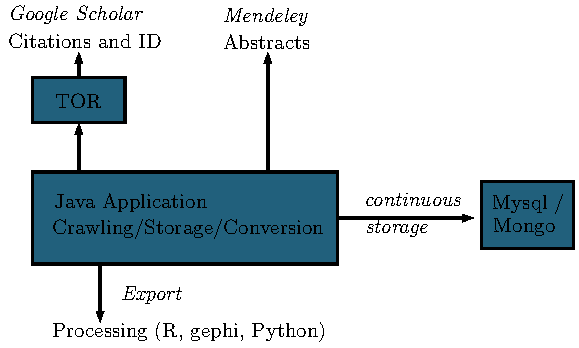
\includegraphics[width=\textwidth]{figures/Fig1.pdf}
\caption{\textbf{Heterogeneous Bibliographical Data Collection and processing.} Architecture of the application for content (semantic data), metadata and citation data collection. The heterogeneity of tasks requires the use of multiple languages : data collection and management is done in Java, and data stored in databases (Mysql and MongoDB) ; data processing is done in python for Natural Language Processing and in R for statistical and network analyses; graph visualizations are done with Gephi software.}
\label{fig:datacollection}
\end{figure}
%%%%%%%%%%%%%%%%%%




%%%%%%%%%%%%%%%%%%
\subsection*{Initial Corpus}

The production database of \textit{Cybergeo} (snapshot taken in February 2016, provided by the editorial board), provides after pre-processing the initial database of articles, with basic information (title, abstract, publication year, authors). The processed version used is available together with the full database constructed, as a \texttt{mysql} dump, at the address given above. This base provide also bibliographical records of articles that give all references cited by the initial base (\emph{forward citations} for the initial corpus).



%%%%%%%%%%%%%%%%%%
\subsection*{Citation Data}

Citation data is collected from \texttt{Google Scholar}, that is the only source for incoming citations~\citep{noruzi2005google} in our case as the journal is poorly referenced in other databases\footnote{or was just added as in the case of \textit{Web of Science}, indexing \textit{Cybergeo} since May 2016 only}. We are aware of the possible biaises using this single source (see e.g.~\cite{bohannon2014scientific})\footnote{or \texttt{http://iscpif.fr/blog/2016/02/the-strange-arithmetic-of-google-scholars}}, but these critics are more directed towards search results or possible targeted manipulations than the global structure of the citation network. The automatic collection requires the use of a crawling software to pipe requests, namely \texttt{TorPool}~\citep{torpool} that provides a Java API allowing an easy integration into our application of data collection. A crawler can therethrough retrieve html pages and get backward citation data, i.e. all citing articles for a given initial article. We retrieve that way two sub-corpuses: references citing papers in \textit{Cybergeo} and references \emph{citing the ones cited} by \textit{Cybergeo}. At this stage, the full corpus contains around $4\cdot10^5$ references.


For the sake of simplicity, we will denote by \emph{reference} any standard scientific production that can be cited by another (journal paper, book, book chapter, conference paper, communication, etc.) and contains basic records (title, abstract, authors, publication year). We work in the following on networks of references, linked by citations.



%%%%%%%%%%%%%%%%%%
\subsection*{Text Data}

A textual description for all references is necessary for a complete semantic analysis. We use for this an other source of data, that is the online catalog of \textit{Mendeley} reference manager software~\cite{mendeley}. It provides a free API allowing to get various records under a structured format. Although not complete, the catalog provides a reasonable coverage in our case, around 55\% of the full citation network. This yields a final corpus with full abstracts of size $2.1\cdot 10^5$. The structure and descriptive statistics of the corresponding citation network is recalled in Fig.~\ref{fig:cybergeo:fig2}.


%\cite{moreno2016uncertainty} no pb of uncertainty : endogenous classification



%%%%%%%%%%%%%%%%%%
\begin{figure}
\centering
%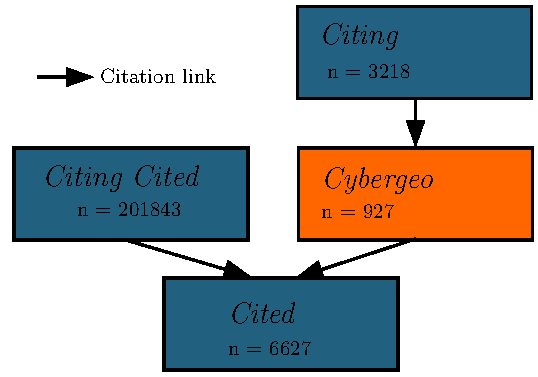
\includegraphics[width=0.6\textwidth]{Figures/Cybergeo/Fig2.pdf}
\includegraphics[width=\linewidth]{Figures/Final/}
\caption{\textbf{Structure and content of the citation network.} The original corpus of \emph{Cybergeo} is composed by 927 articles, themselves cited by a slightly larger corpus (yielding a stationary impact factor of around 3.18), cite $\simeq 6600$ references, themselves co-cited by more than $2\cdot 10^5$ works for which we have a textual description.\label{fig:cybergeo:fig2}}{\textbf{Structure et contenu du réseau de citation.}\label{fig:cybergeo:fig2}}
\end{figure}
%%%%%%%%%%%%%%%%%%









%%%%%%%%%%%%%%%%%%
\subsection{Methods and Results}{Méthodes et Résultats}
%%%%%%%%%%%%%%%%%%



%%%%%%%%%%%%%%%%%%
\subsubsection{Citation Network Properties}{Propriétés du réseau de citation}

\paragraph{Properties}{Propriétés}

% mean(degree(gcitation,which(degree(gcitation,mode="in")>0),mode="in"))
%[1] 121.5615

As detailed above, we are able by the reconstruction of the citation network at depth $\pm 1$ from the original $927$ references of the journal to retrieve around $45\cdot 10^6$ references, on which $2.1\cdot 10^5$ have an abstract text allowing semantic analysis. A first glance on citation network properties provides useful insights. Mean in-degree (that can be interpreted as a stationary integrated impact factor) on references for which it can be defined has a value of $\bar{d}=121.6$, whereas for articles in \textit{Cybergeo} we have $\bar{d}=3.18$. This difference suggests a variety for status of references, from old classical works (the most cited has 1051 incoming citations) to recent less influential works.


%%%%%%%%%%%%%%%%%
\begin{figure}
%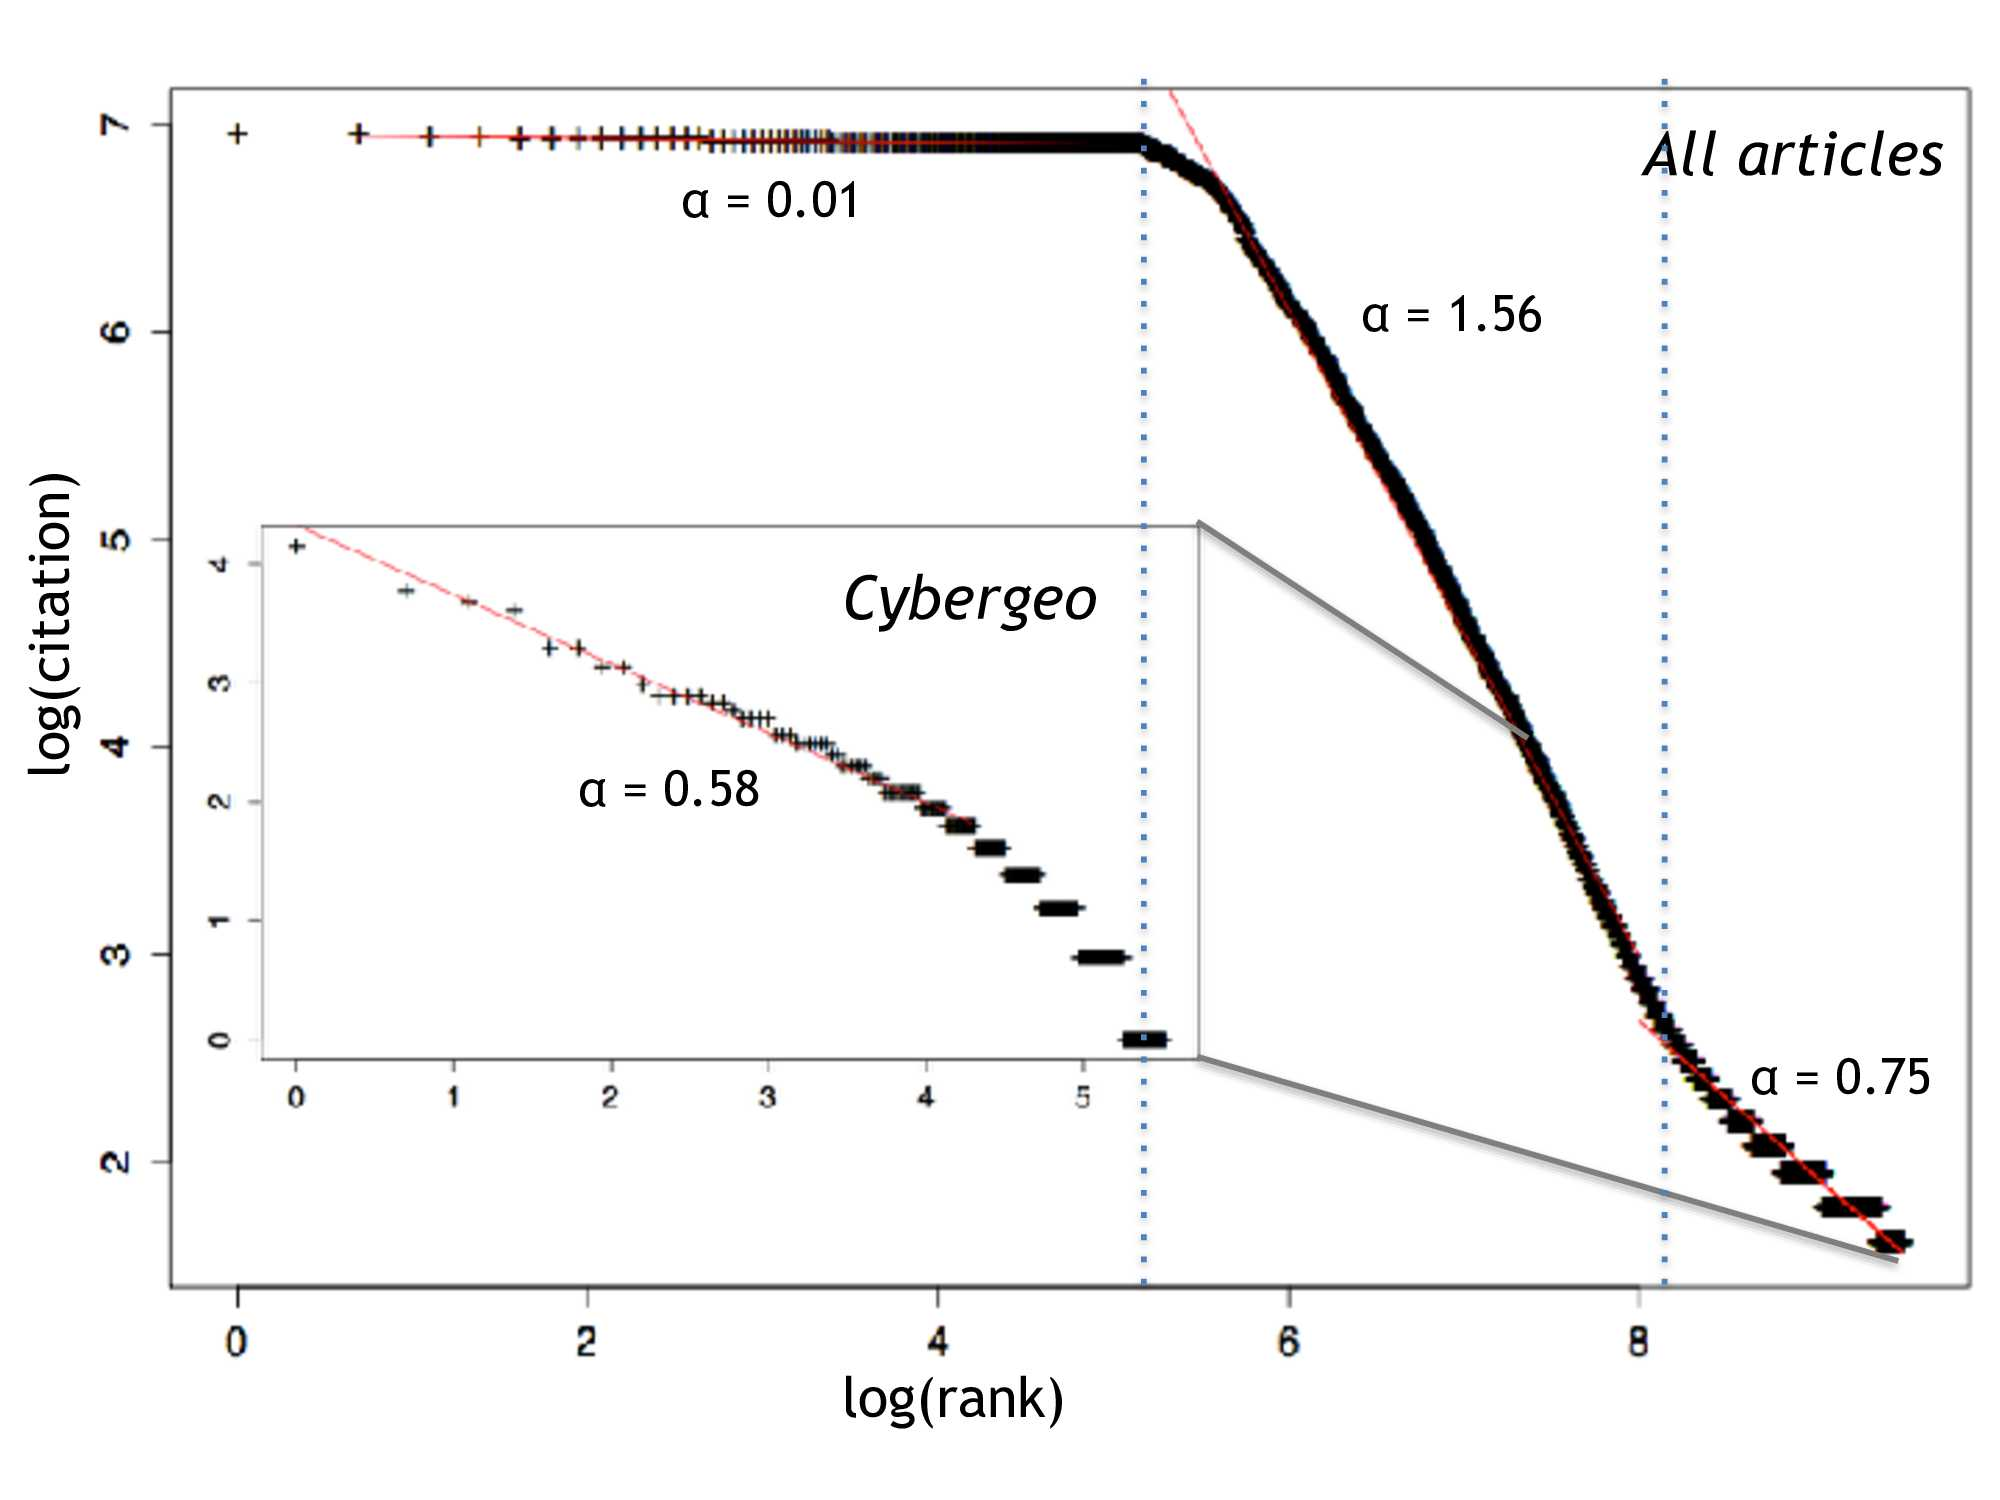
\includegraphics[width=\textwidth]{Figures/Cybergeo/Fig3.jpg}
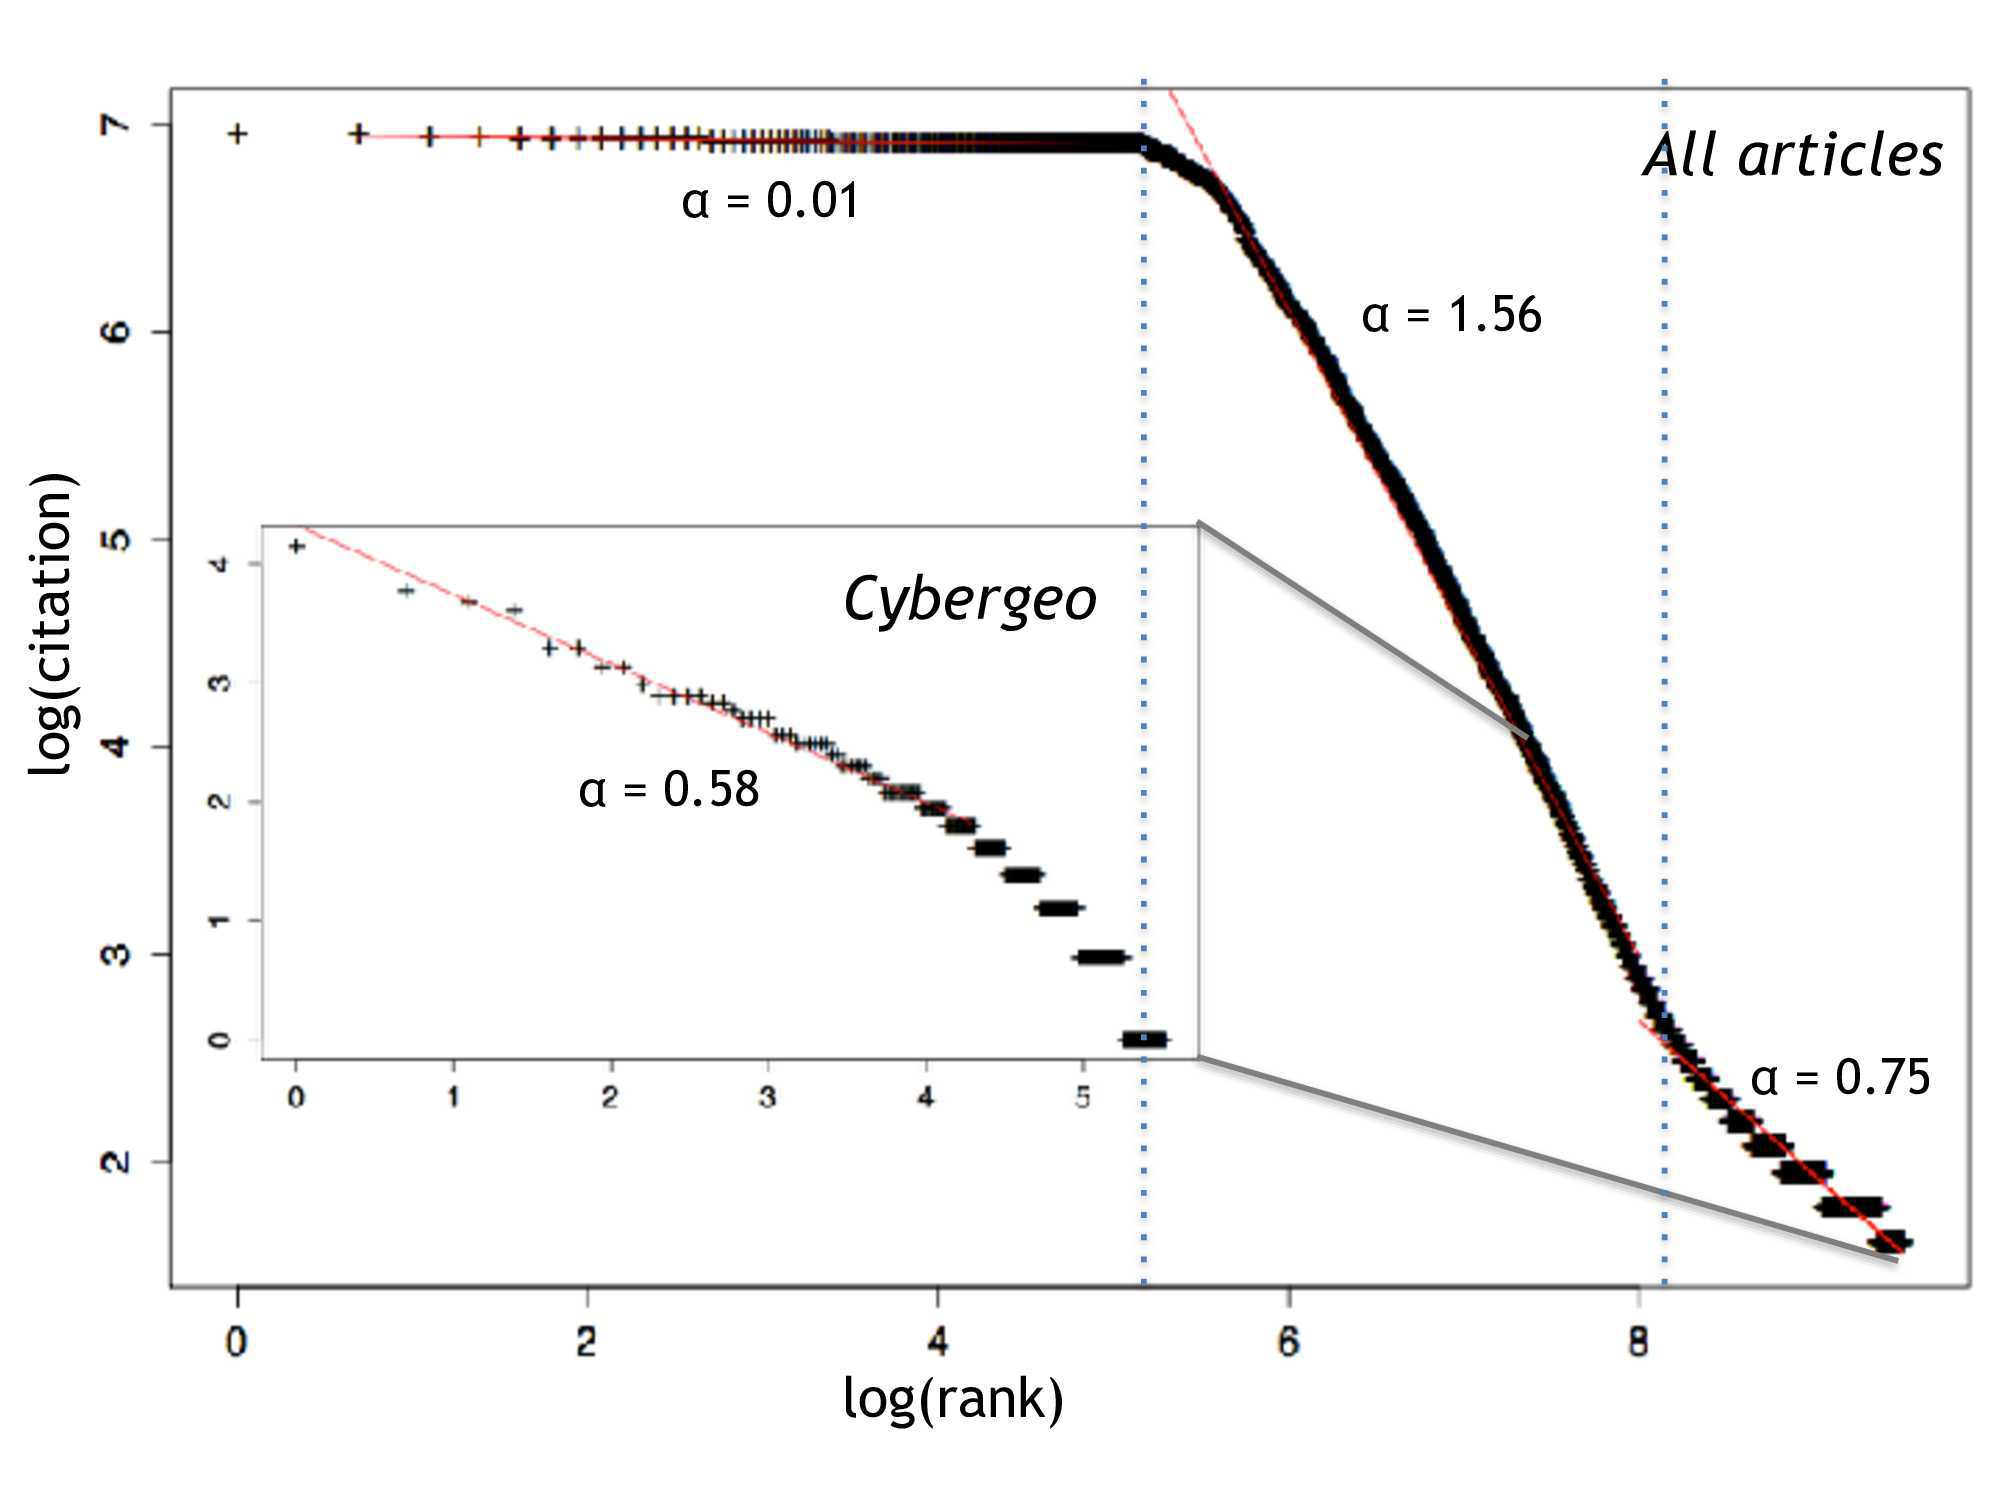
\includegraphics[width=\linewidth]{Figures/Final/B-cybergeo-fig3.jpg}
\caption{\textbf{Rank-size plot of citations received.} The plot unveils three superposed citations regimes, corresponding to power laws with different levels of hierarchy. The references in \textit{Cybergeo} (inset plot) are themselves in the tail and less hierarchical.\label{fig:cybergeo:fig3}}{\textbf{Graphe rang-taille des citations reçues.}\label{fig:cybergeo:fig3}}
\end{figure}
%%%%%%%%%%%%%%%%%


This diversity is confirmed by the hierarchical organisation examined in Fig.~\ref{fig:cybergeo:fig3} that unveils three superposed regimes. More precisely, we look at the rank-size plot, given by the logarithm of the number of citations received as a function of the rank of the paper. We find, as expected~\citep{redner1998popular}, localized power-law behaviors. A first set of around 150 references shows a very low hierarchy (rank-size exponent $\alpha = 0.01$) and corresponds to classical references in different disciplines. A second regime ($\alpha = 1.56$) is much more hierarchized, followed by a last regime less hierarchical ($\alpha = 0.75$) containing more recent papers (average publication year mid-2005, against mid-1998 for the second and 1983 for the first).



Other topological properties reveal typical patterns of citation practices: for example, the existence of high-order cliques (complete sub-networks) implies citation practices which compatibility with the cumulative nature of knowledge may be questionable~\cite{pumain2005cumulativite}, since these need always to source back the production of knowledge in the most recent works. An exemple of such a clique in shown in Fig.~\ref{fig:cybergeo:fig4}.



%%%%%%%%%%%%%%%%%
\begin{figure}
%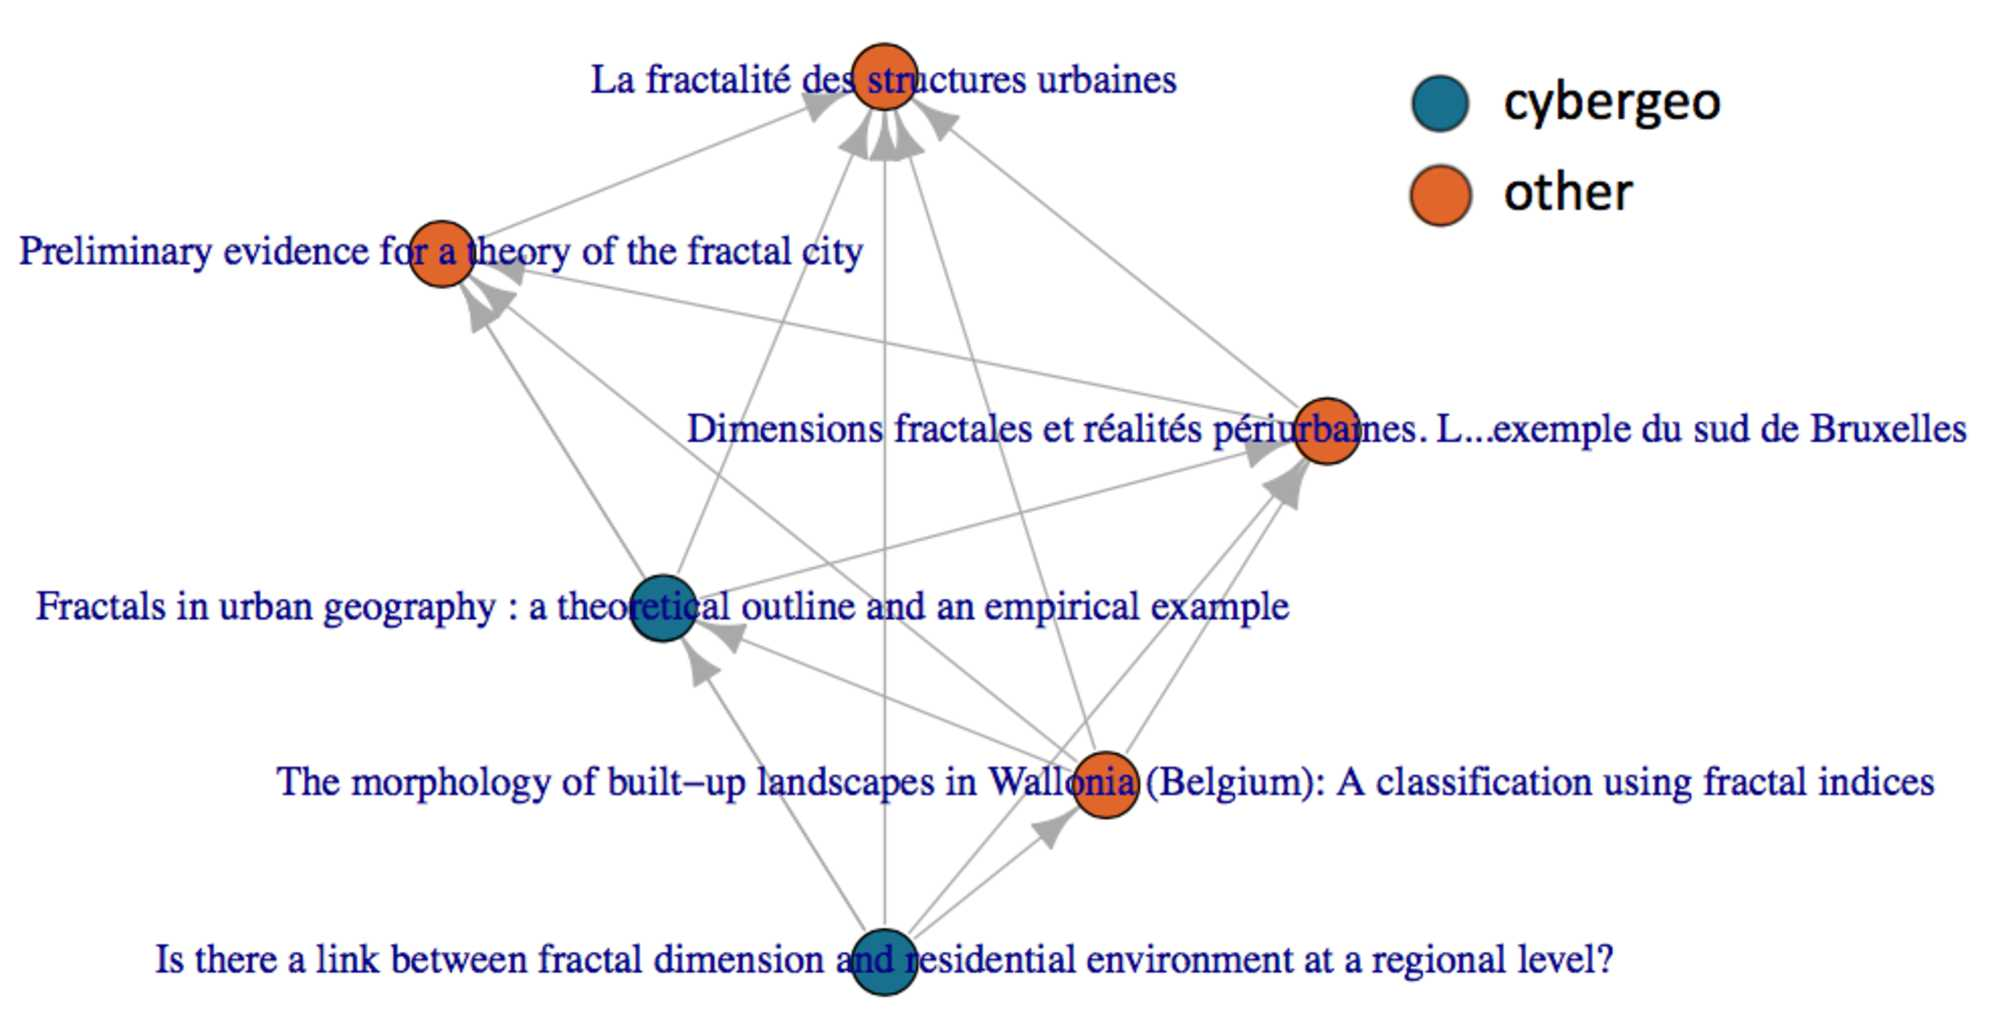
\includegraphics[width=\textwidth]{Figures/Cybergeo/Fig4.jpg}
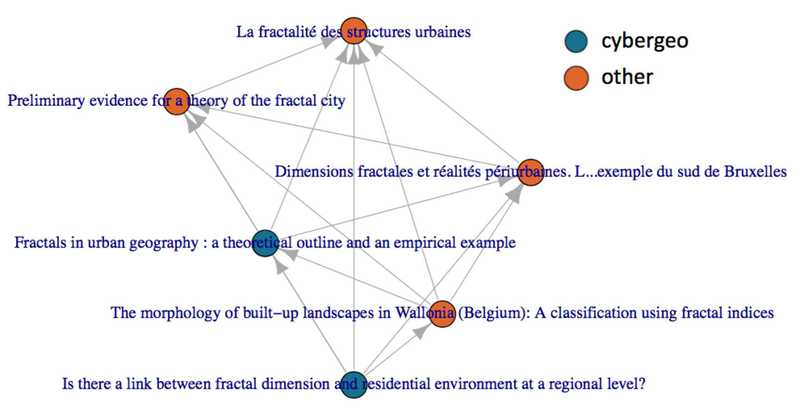
\includegraphics[width=\linewidth]{Figures/Final/B-cybergeo-fig4.jpg}
\caption{Example of a maximal clique in the citation network, paper of \texttt{cybergeo} being in blue. Such topological structure reveal citation practices such as here a systematic citation of previous works in the research niche.\label{fig:cybergeo:fig4}}{\textbf{Exemple d'une clique maximale dans le réseau de citation.}\label{fig:cybergeo:fig4}}
\end{figure}
%%%%%%%%%%%%%%%%%



\paragraph{Citation communities}{Communautés de citation}

The citation network is a first opportunity to construct endogenous disciplines, by extracting citation communities. More precisely, this step aims at finding recurrent patterns in citations that would define a field by its citation practices. In order to be consistent with the particular data structure we have (missing incoming citations for sub-corpuses at maximal depth), we filter the network by removing all nodes with degree smaller than one. This ensures that kept nodes are either at least cited by an other node (and thus there are no missing edges for these nodes) or cite at least two other nodes, what can make ``bridges'' between sub-communities. The resulting network has a size of $\left|V\right| = 107164$ nodes and $\left|E\right| = 309778$ edges. It is visualized in Fig.~\ref{fig:cybergeo:fig5}.



%%%%%%%%%%%%%%%%%
\begin{figure}
%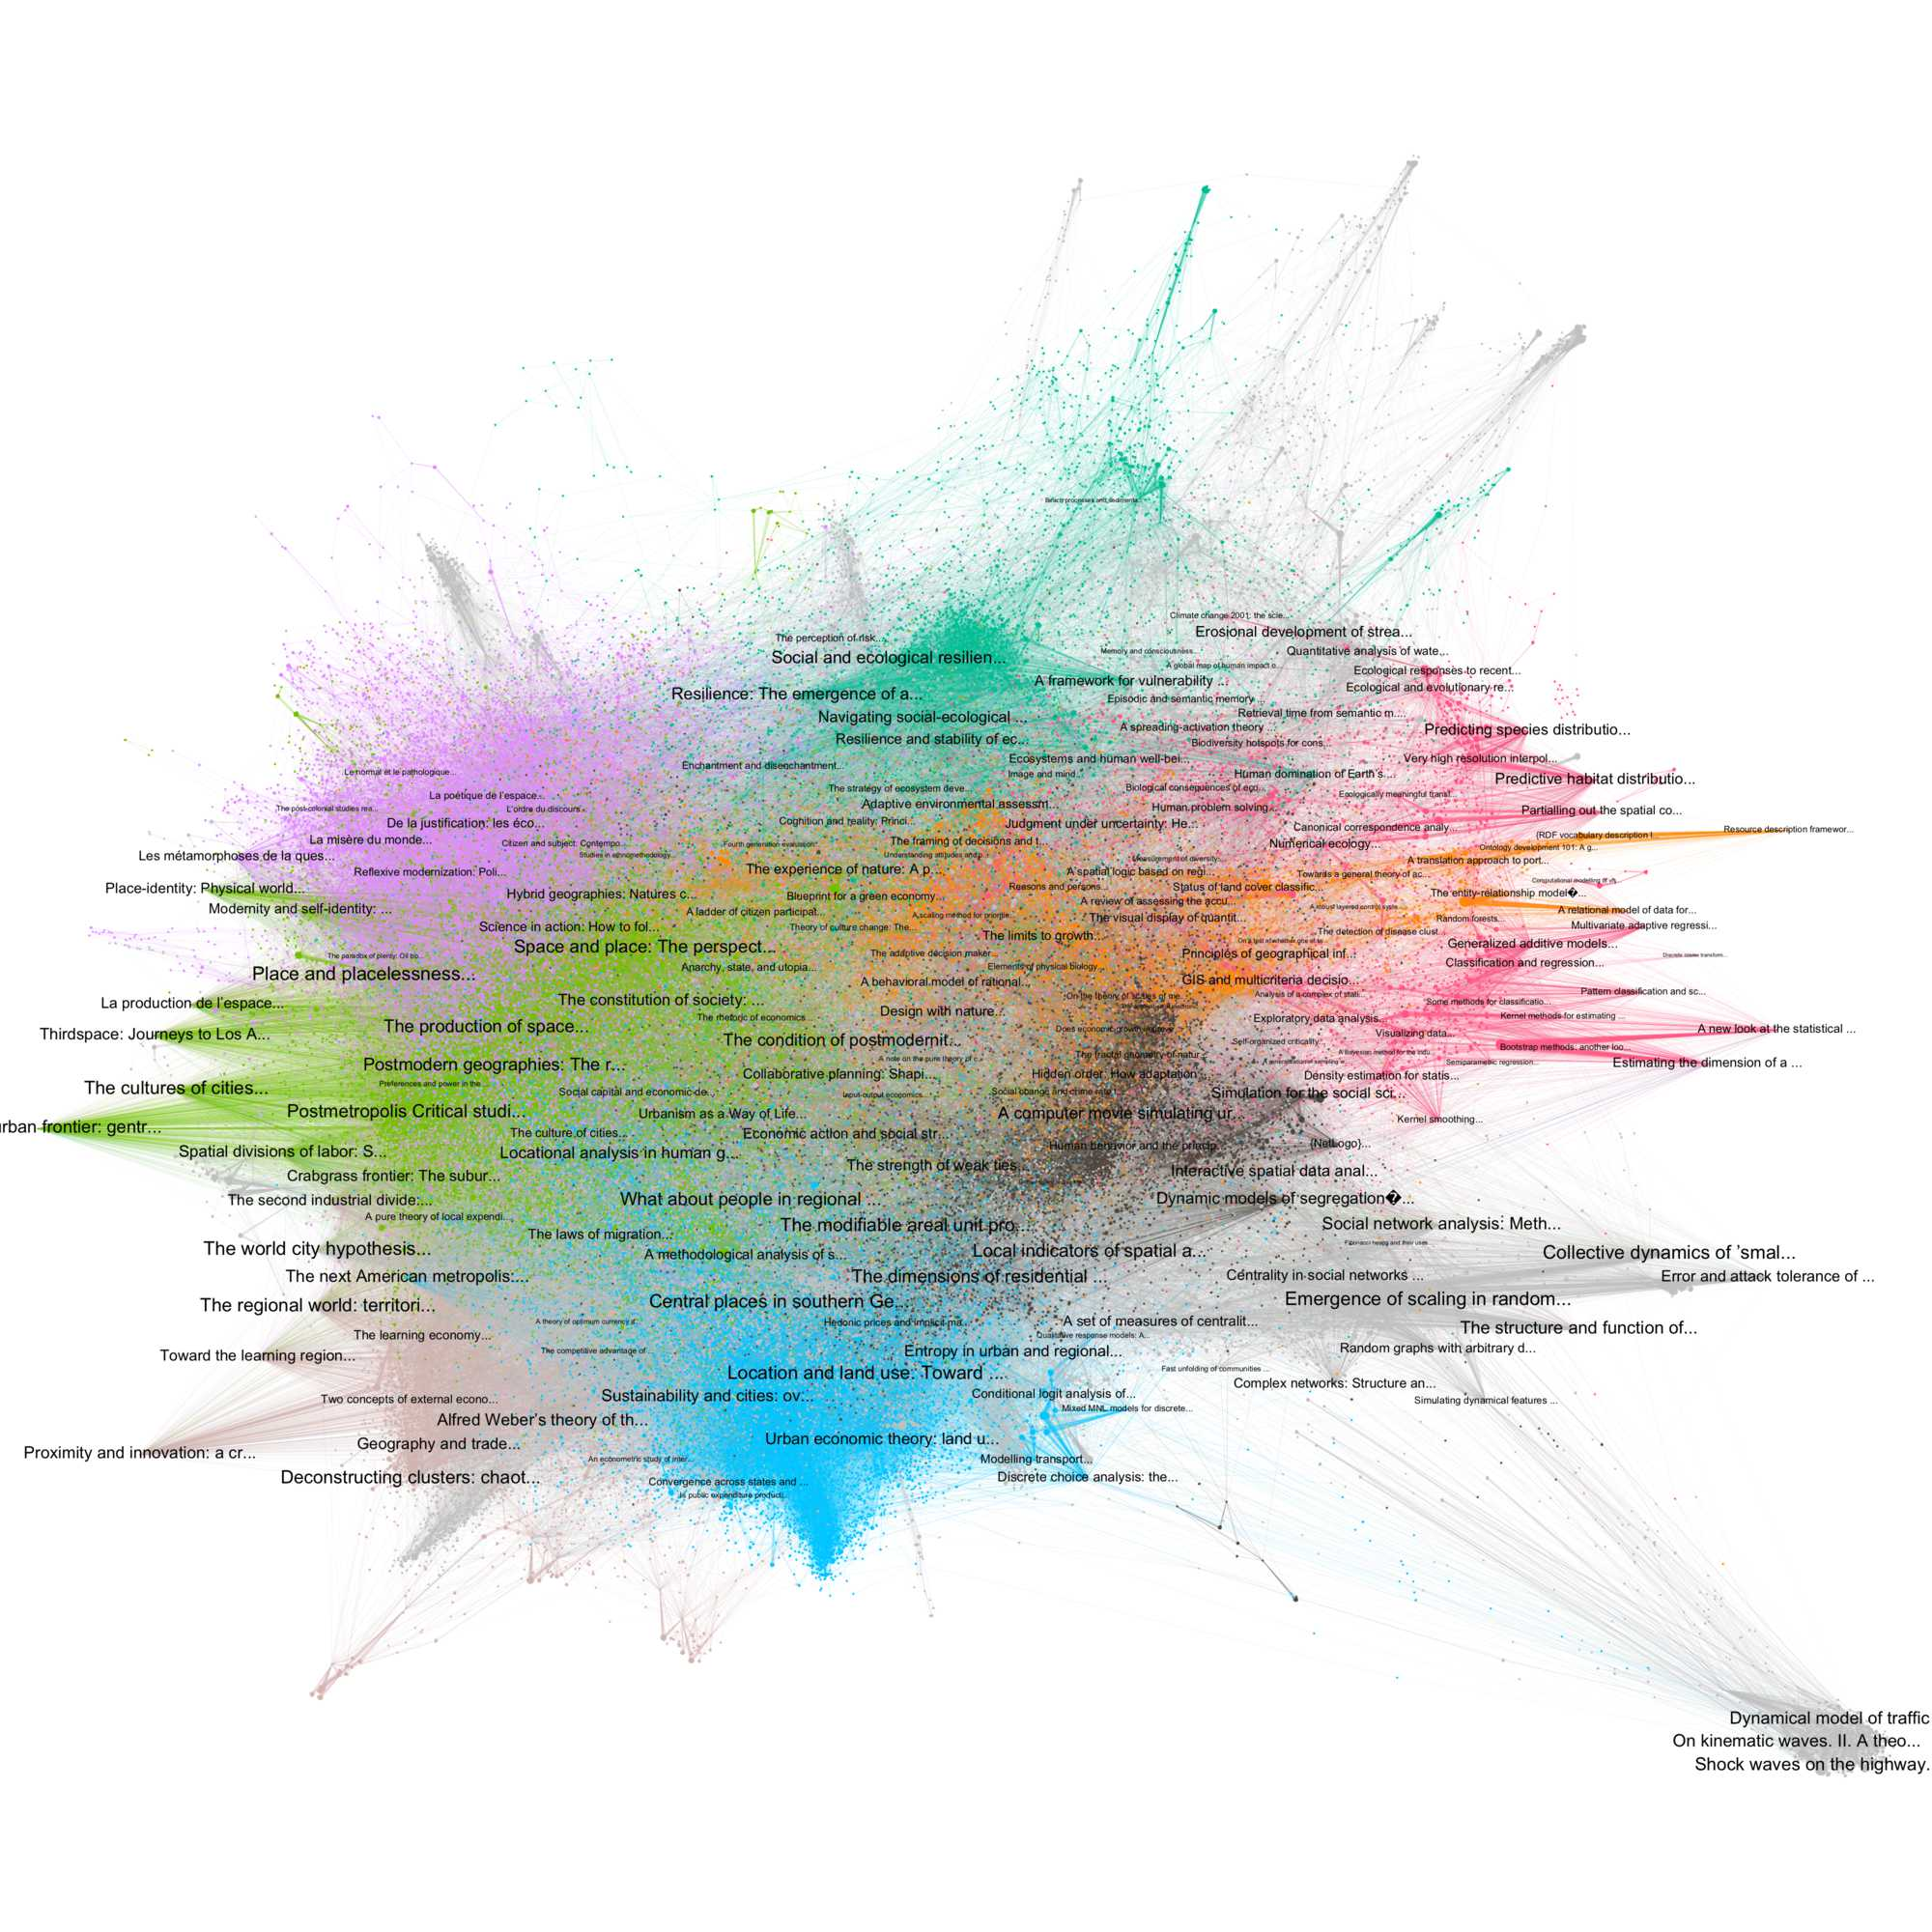
\includegraphics[width=\textwidth]{Figures/Cybergeo/Fig5.jpg}
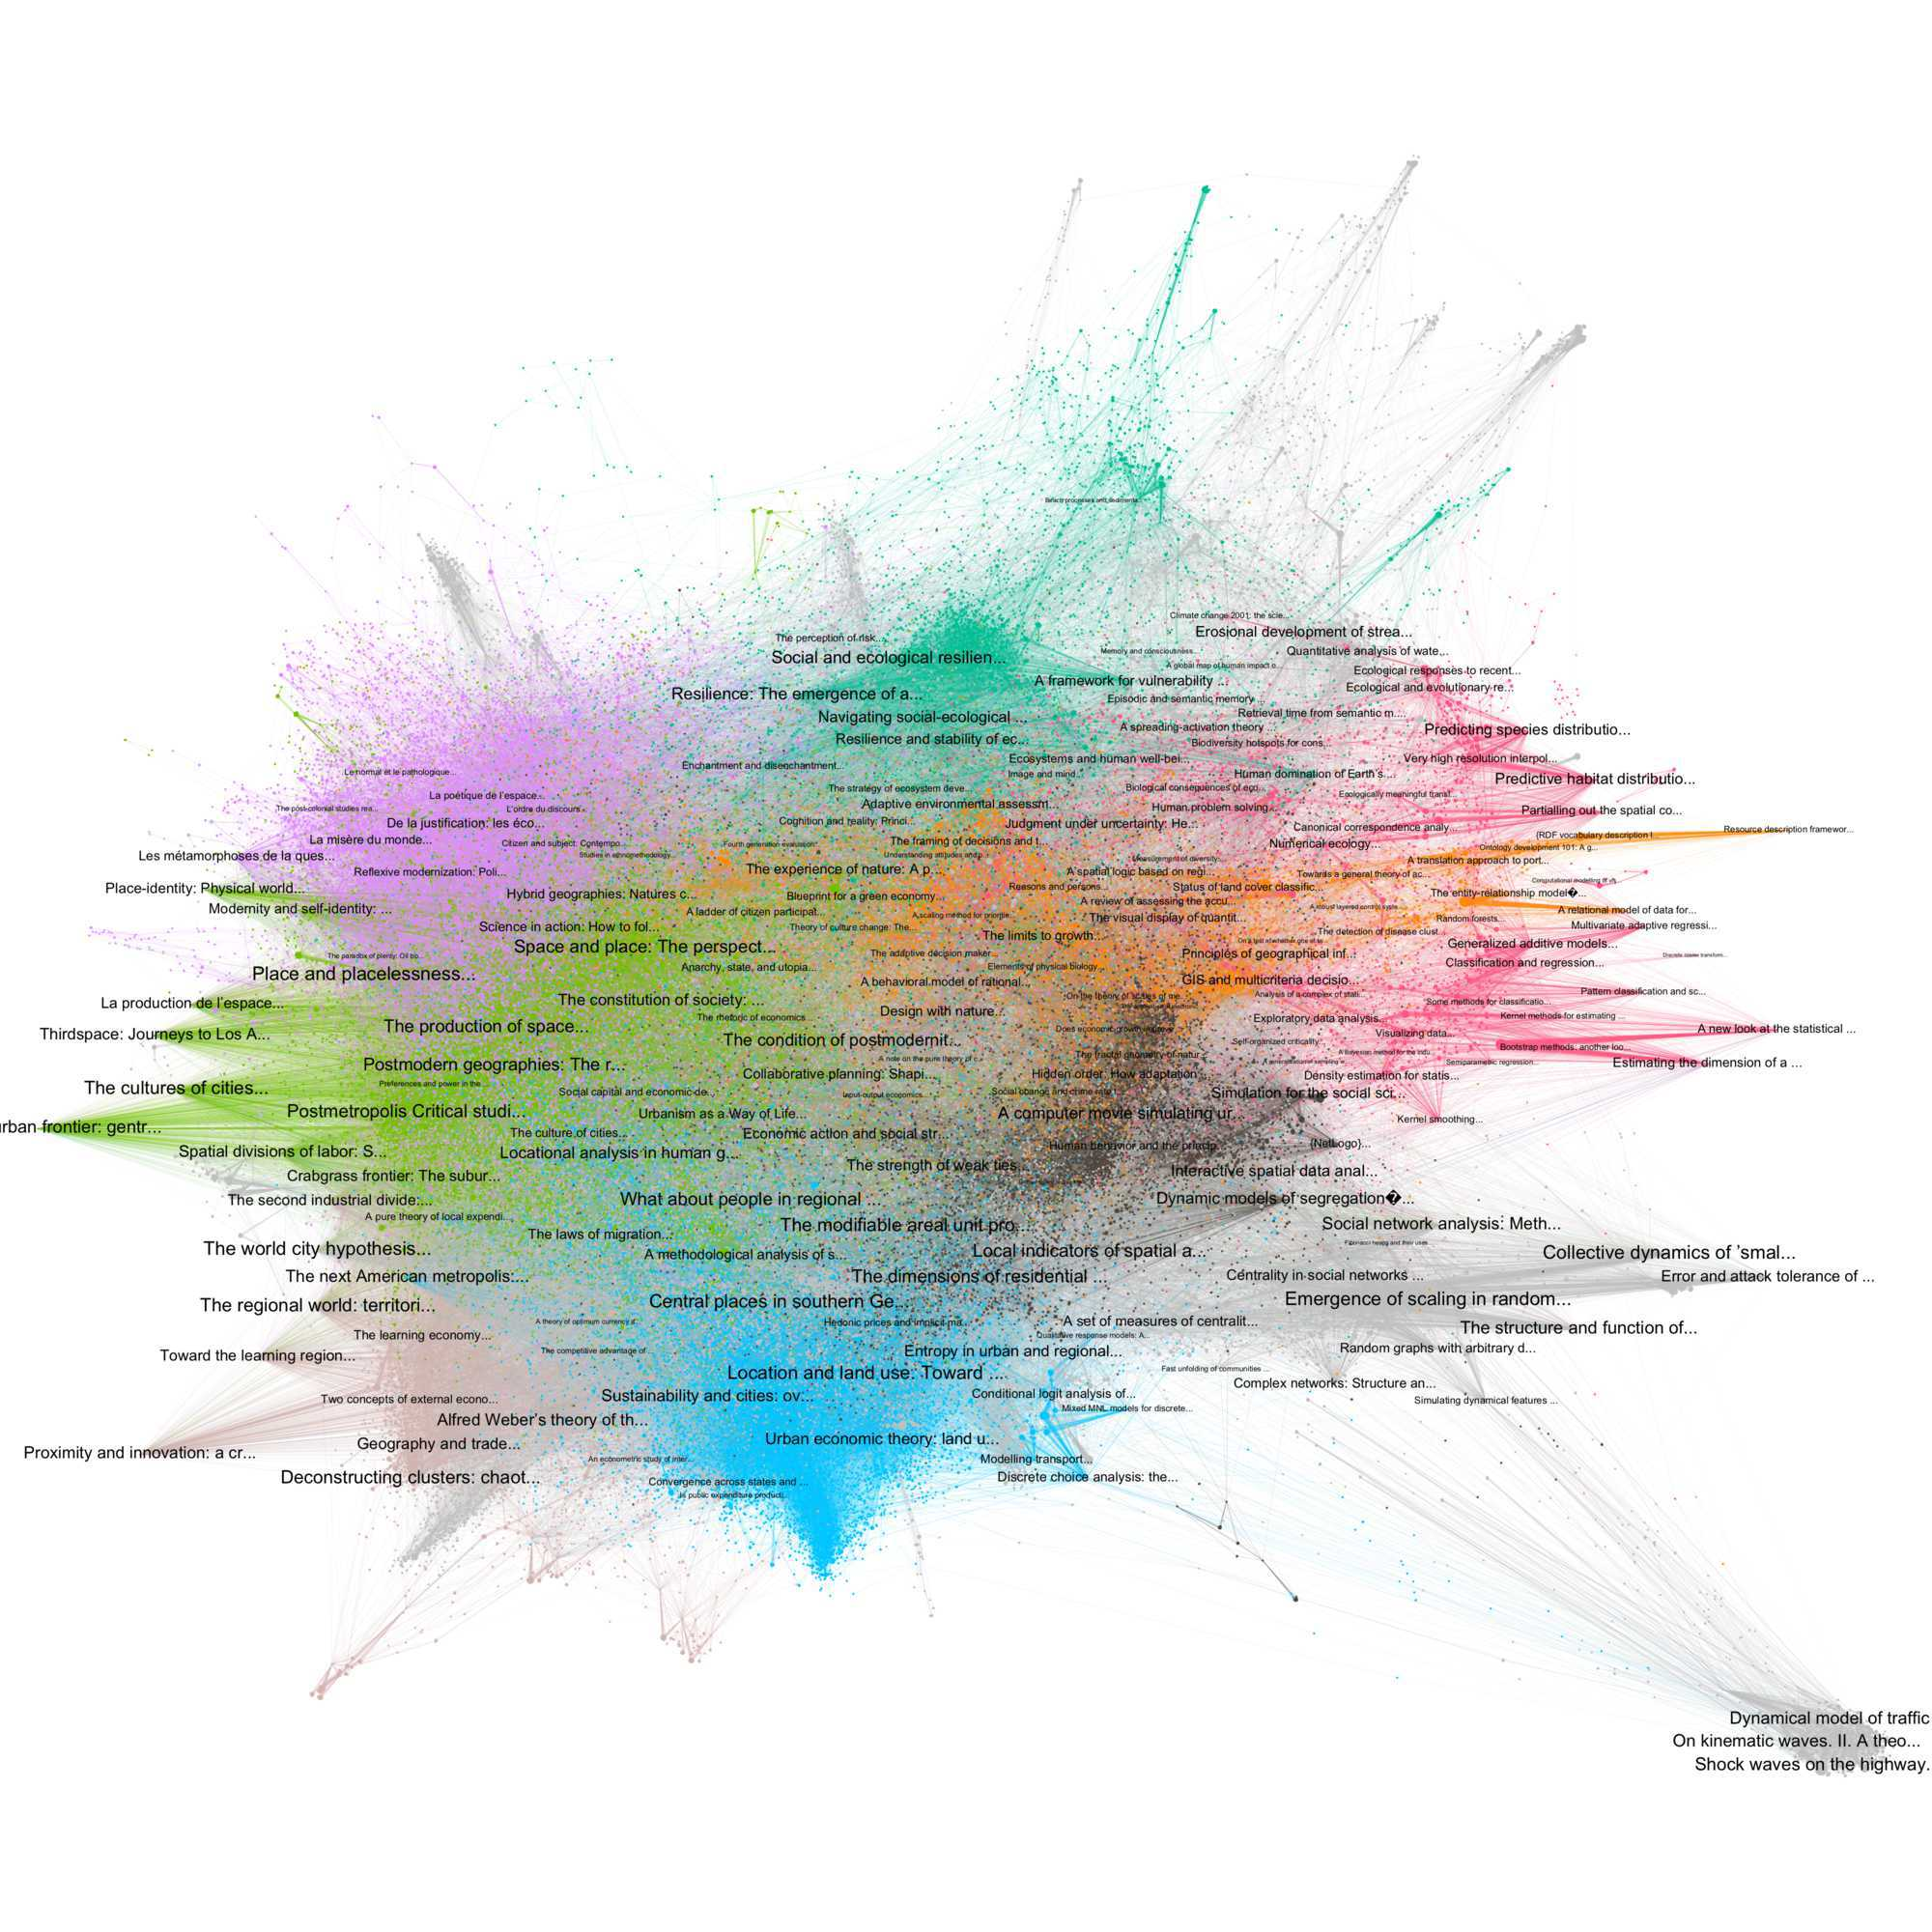
\includegraphics[width=\linewidth]{Figures/Final/B-cybergeo-fig5.jpg}
\caption{\textbf{Citation Network.} We show only the ``core'' of the citation network, composed by references with a degree larger than one ($\left|V\right| = 107164$ and $\left|E\right| = 309778$). The community detection algorithm provides 29 communities with a modularity of 0.71. Nodes and edges color gives the main community (for example ecology in magenta, GIS in orange, Socio-ecology in turquoise, Social geography in green, Spatial analysis in blue). Node labels give shortened titles of most cited papers, size is scaled according to their in-degree. The graph is spatialized using a Force-Atlas algorithm.\label{fig:cybergeo:fig5}}{\textbf{Réseau de citations.}\label{fig:cybergeo:fig5}}
\end{figure}
%%%%%%%%%%%%%%%%%


We use a standard modularity optimization algorithm to identify communities~\citep{blondel2008fast} in this citation network. It provides 29 communities with a modularity of 0.71. In comparison, a bootstrap of 100 randomisations of links in the network gives an average modularity of $-1.0\cdot 10^{-4} \pm 4.4\cdot 10^{-4}$ which means that communities are highly significant.


We name the communities by inspection of the titles of most cited references in each. The 14 communities that have a size larger than 2.5\% of the network are : Complex Networks, Ecology, Social Geography, Sociology, GIS, Spatial Analysis, Agent-based Modeling and Simulation (ABMS), Socio-ecology, Urban Networks, Urban Simulation, Urban Studies, Economic Geography, Accessibility/Land-use, Time Geography. These categories do not directly correspond to well-defined disciplines, as some correspond more to methods (ABMS), objects of study (Urban Studies), or paradigms (Complex Networks). Some are ``specializations'' of others : most papers in Urban Studies can also be classified as Critical and Social geography. This way, we construct endogenous disciplines that correspond to \emph{scientific practices} (what is cited) more than their representation (the ``official'' disciplines). The relative positioning of communities in Fig.~\ref{fig:cybergeo:fig5}, obtained with a Force-Atlas algorithm, tells a lot about their respective relations : for example, social geography makes a bridge between Urban Studies and Economic Geography, whereas the connection between Socio-ecology and Urban simulations is done by GIS (what can be expected as geomatics is an interdisciplinary field). GIS also separates and connects two subfield of Ecology, on one side more thematic studies on ecological habitats, and on the other sides statistical methods. These relations already inform qualitatively patterns of interdisciplinarity, in the sense of integration measures. We will also in the following use these communities to situate the semantic classification.





%%%%
% Core properties :
% |V| = 107164
% |E| = 309778
% Modularity = 0.694



% "Community 24 ; corpus prop 2.12291441155612"
%17103773263010692469                                             Shock waves on the highway    704
%5930190645967036557                              Traffic dynamics: studies in car following    531
%6454619432004957861  On kinematic waves. II. A theory of traffic flow on long crowded roads    671
%15823582570548231219         Dynamical model of traffic congestion and numerical simulation    673
%[1] "Community 10 ; corpus prop 4.16557799260946"
%15243168274213127296                  Social network analysis: Methods and applications    658
%10638755925462666384                            Emergence of scaling in random networks    756
%4992186057191694547  Collective dynamics of \342\200\231small-world\342\200\231networks    758
%12945060519911641528                     The structure and function of complex networks    687
%[1] "Community 16 ; corpus prop 4.81318353178306"
%13398523337335518206                         Predictive habitat distribution models in ecology    566
%13467121252331935431                                               Generalized additive models    418
%11029642873510533673 Predicting species distribution: offering more than simple habitat models    562
%13831040667378725133                                       Estimating the dimension of a model    454
%[1] "Community 17 ; corpus prop 11.8743234668359"
%6052144816936635558                                        Pour une g\303\251ographie du pouvoir    478
%9980715752622498273                      Les mots de la g\303\251ographie: dictionnaire critique    590
%14304156646457097003                    De la justification: les \303\251conomies de la grandeur    440
%2870436522105960522   Les m\303\251tamorphoses de la question sociale: une chronique du salariat    458
%[1] "Community 18 ; corpus prop 5.57556642155948"
%6414662845457641721   The constitution of society: Outline of the theory of structuration    593
%4337430435041504651  Modernity and self-identity: Self and society in the late modern age    493
%7898783771677764446                                        The condition of postmodernity    658
%7835092538327027347     Economic action and social structure: the problem of embeddedness    516
%[1] "Community 6 ; corpus prop 3.60475532828189"
%                                                          titles degree
%12482866708510596998                           The power of maps    575
%1164911542533093357      GIS and multicriteria decision analysis    463
%16457974396311846489  Spatial behavior: A geographic perspective    552
%2954521275884877195                       Deconstructing the map    631
%[1] "Community 3 ; corpus prop 5.13885259975365"
%11531103519383816169 The structure and growth of residential neighborhoods in American cities    692
%62057246354689685                                                        The nature of cities    713
%3545913291616437667                                   Locational analysis in human geography.    627
%17899222184184316747                                       Central places in southern Germany    740
%[1] "Community 14 ; corpus prop 6.66735097607405"
%12954335397668543979  Cellular automata and fractal urban form: a cellular modelling approach to the evolution of urban land-use patterns
%4133663650988164381                                                                       Fractal cities: a geometry of form and function
%1594743421920318397                                                       Growing artificial societies: social science from the bottom up
%14559759739366955015                                   Multi-agent systems for the simulation of land-use and land-cover change: a review
%                     degree
%12954335397668543979    743
%4133663650988164381     747
%1594743421920318397     604
%14559759739366955015    778
%[1] "Community 9 ; corpus prop 1.9829420327722"
%1594126764449801706                                                               Quantitative analysis of watershed geomorphology
%8328827169345207094  Erosional development of streams and their drainage basins; hydrophysical approach to quantitative morphology
%8539006751955791402                                                                              Statistical law of stream numbers
%12081487864131557751                                                  Hypsometric (area-altitude) analysis of erosional topography
%                     degree
%1594126764449801706     382
%8328827169345207094     536
%8539006751955791402     391
%12081487864131557751    408
%[1] "Community 27 ; corpus prop 0.851032063006233"
%10726714213083688457                                Transmission dynamics of the etiological agent of SARS in Hong Kong: impact of public health interventions
%3970869213781401070  Impact of climatic change on the northern latitude limit and population density of the disease-transmitting European tick Ixodes ricinus.
%2455775719744402150                                   Epidemiological determinants of spread of causal agent of severe acute respiratory syndrome in Hong Kong
%8395695762893339661                                                                     Transmission dynamics and control of severe acute respiratory syndrome
%                     degree
%10726714213083688457    475
%3970869213781401070     116
%2455775719744402150     216
%8395695762893339661     430
%[1] "Community 8 ; corpus prop 0.733455264827741"
%932712685133827561   The physiological equivalent temperature\342\200\223a universal index for the biometeorological assessment of the thermal environment
%1480142480183496272                                                                                                                      The urban climate
%17024728103875347383                             A field study of thermal comfort in outdoor and semi-outdoor environments in subtropical Sydney Australia
%833745332327046870                                                         Applications of a universal thermal index: physiological equivalent temperature
%                     degree
%932712685133827561      391
%1480142480183496272     173
%17024728103875347383    153
%833745332327046870      293
%[1] "Community 21 ; corpus prop 6.45272666193871"
%12312403172976436756                                          Social and ecological resilience: are they related?
%932477214288257460   Resilience: The emergence of a perspective for social\342\200\223ecological systems analyses
%5340448582567072501                                     From metaphor to measurement: resilience of what to what?
%1509391713535671469           Navigating social-ecological systems: building resilience for complexity and change
%                     degree
%12312403172976436756    665
%932477214288257460      646
%5340448582567072501     651
%1509391713535671469     579
%[1] "Community 13 ; corpus prop 3.00474039789482"
%                                                           titles degree
%12568908445725112885                             The world cities    629
%14432190559149797085                     A roster of world cities    581
%3966620121471250312   World city network: a global urban analysis    716
%7479248257935000396                     The world city hypothesis    760
%
%[1] "Community 23 ; corpus prop 5.62875592549737"
%3553655105619346230                                                                  The modifiable areal unit problem
%14305556346317738837  A million or so correlation coefficients: three experiments on the modifiable areal unit problem
%15192663253141002697                                    A computer movie simulating urban growth in the Detroit region
%2556056281630746501                                                       Local indicators of spatial association-LISA
%                     degree
%3553655105619346230     741
%14305556346317738837    661
%15192663253141002697    643
%2556056281630746501     724
%[1] "Community 2 ; corpus prop 9.9660333694151"
%                                                                        titles degree
%12738968557765837578                                    The cultures of cities    732
%13746171706822239563     Postmetropolis Critical studies of cities and regions    715
%2116873643451406893   Fortress America: gated communities in the United States    704
%14292387866086321708                                   Place and placelessness    760
%[1] "Community 22 ; corpus prop 7.13579187040424"
%                                                                              
%11080283063311825032  The regional world: territorial development in a global economy    740
%3554088320531351693                                        Location and space-economy    719
%7086787680145296542       Deconstructing clusters: chaotic concept or policy panacea?    726
%[1] "Community 28 ; corpus prop 1.4379829047068"
%
%16044574669948655149     Saharan dust contributions to PM10 and TSP levels in Southern and Eastern Spain
%8425362340869409578   Climats, for\303\252ts et d\303\251sertification de l\342\200\231Afrique tropicale
%1129714354835431503                                                    Nonparametric tests against trend
%1135676043916984792                                A non-parametric approach to the change-point problem
%                     degree
%16044574669948655149    144
%8425362340869409578     160
%1129714354835431503     181
%1135676043916984792     203
%[1] "Community 1 ; corpus prop 1.67500279944758"
%                                                               titles degree
%1627107393903704279         The dimensions of residential segregation    724
%4099483990695182730                             Models of segregation    466
%747074237233961749          Dynamic models of segregation\342\200\240    622
%18105468109972109903 A methodological analysis of segregation indexes    506
%[1] "Community 5 ; corpus prop 9.77847038184465"
%                                                                           titles degree
%13956442331799241731 Location and land use. Toward a general theory of land rent.    748
%15575741556156415962                            How accessibility shapes land use    782
%13897256231045447464                                      Urban spatial structure    783
%5192159686471589942                 Are compact cities a desirable planning goal?    741
%[1] "Community 26 ; corpus prop 1.98760777873166"
%12131824341349033633                                              Connectivity is a vital element of landscape structure
%15969739511774356860      The application of \342\200\231least-cost\342\200\231modelling as a functional landscape model
%3875238890909508946  Promoting ecosystem and human health in urban areas using green infrastructure: a literature review
%15970185536531379583                                                                   Ecosystem services in urban areas
%                     degree
%12131824341349033633    343
%15969739511774356860    262
%3875238890909508946     265
%15970185536531379583    319
%[1] "Community 4 ; corpus prop 1.24575417117689"
%                                                                      titles degree
%17518815146409301085                       Visual methods in social research    309
%3130282044894438080                 Image as a factor in tourism development    222
%6005112106352993762   Understanding and measuring tourist destination images    211
%17773583015280146421    Talking about pictures: A case for photo elicitation    412
%
%[1] "Community 11 ; corpus prop 2.66134149527827"
%15987432381426193038                                                                                           Time in geographic information systems
%4916773650386052166  It\342\200\231s about time: A conceptual framework for the representation of temporal dynamics in geographic information systems
%10741249551199253506                                                                                 A spatial logic based on regions and connection.
%1707686457311089380                                       An event-based spatiotemporal data model (ESTDM) for temporal analysis of geographical data
%                     degree
%15987432381426193038    557
%4916773650386052166     399
%10741249551199253506    339
%1707686457311089380     388
%[1] "Community 12 ; corpus prop 0.0541226531297824"
%
%320633167171028945   \342\200\231Unite Unite Europe\342\200\231The political and cultural structures of Europe as reflected in the Eurovision Song Contest
%8402251348308572830          Comparison of Eurovision Song Contest simulation with actual results reveals shifting patterns of collusive voting alliances.
%2610553645533349879                                                       Save the last dance for me: Unwanted serial position effects in jury evaluations
%10488781352782564265                                                  Save the last dance II: Unwanted serial position effects in figure skating judgments
%                     degree
%320633167171028945       25
%8402251348308572830      24
%2610553645533349879      32
%10488781352782564265     18
%[1] "Community 25 ; corpus prop 0.747452502706133"
%                                                         titles degree
%5749645930528845292           Theorising the rise of regionness     89
%16110139515439702034          The geographical pivot of history    232
%18249508238183354137                            Arctic meltdown     57
%15128616333100707022  Geography and politics in a world divided    112
%[1] "Community 29 ; corpus prop 0.570154156246501"
%
%17875356408399137122 The second demographic transition in Western countries: An interpretation    361
%9773560585688720648                          Europe\342\200\231s second demographic transition    422
%4173326927865475733              La famille en Europe occidentale: divergences et convergences     79
%5987517425216101496                        Family ties in Western Europe: persistent contrasts    248
%[1] "Community 20 ; corpus prop 0.0718524877757456"
%                                                                                                                                    
%18395417624936874618                                                                The development crisis in Vietnam\342\200\231s mountains
%269325805179871458    Doi Moi in the mountains: land use changes and farmers\342\200\231 livelihood strategies in Bac Kan Province, Viet Nam
%8071930996413902082                                                                   Choosing rural road investments to help reduce poverty
%5647127754479004480                                           The spatial distribution of poverty in Vietnam and the potential for targeting
%                     degree
%18395417624936874618     29
%269325805179871458       37
%8071930996413902082      34
%5647127754479004480      17
%
%[1] "Community 7 ; corpus prop 0.0261281773729984"
%5883716409547177886 All or none: no stable hybrid or half-way solutions for launching the learned periodical literature into the postGutenberg galaxy
%9133434386405239110                                                                                         Web journals publishing: a UK perspective
%6281042621755024923                                                                                                 The invisible hand of peer review
%2432100162443594098                                                                             Electronic publishing takes journals into a new realm
%                    degree
%5883716409547177886     19
%9133434386405239110      5
%6281042621755024923     18
%2432100162443594098      4
%
%[1] "Community 15 ; corpus prop 0.0083983427270352"
%[1] titles degree
%<0 rows> (or 0-length row.names)
%
%[1] "Community 19 ; corpus prop 0.0177298346459632"
%15912331793517931633 Les discriminations selon l\342\200\231origine dans l\342\200\231acc\303\250s aux soins
%2939440609801692906                          Etat de sant\303\251 des populations immigr\303\251es en France
%695207205763025392                                         Entre droit aux soins et qualit\303\251 des soins
%1837393795895317408               Sant\303\251 et immigration. Les v\303\251rit\303\251s politiques du corps
%                     degree
%15912331793517931633      7
%2939440609801692906       5
%695207205763025392        5
%1837393795895317408       5
%
%










%%%%%%%%%%%%%%%%%%
\subsubsection{Semantic Communities Construction}{Construction des communautés sémantiques}

We now turn to the methodological details for the construction of the semantic classification. This step adapts the methodology described by~\cite{bergeaud2017classifying}, who construct a semantic classification on patent data.

%%%%%%%%%%%%%%%%%%
\paragraph{Relevant Keywords Extraction}{Extraction des Mots-clés pertinents}

We recall that our corpus with available text consists of around $2\cdot 10^5$ abstracts of publications at a topological distance shorter than 2 from the journal \textit{Cybergeo} in the citation network. The first important step is to extract relevant keywords from abstracts. Text processing is done with the python library \texttt{nltk}~\citep{bird2006nltk}. We add a particular treatment to the method of~\cite{bergeaud2017classifying}, as our corpus is multilingual: language detection is done with the technique of \emph{stop-words}~\citep{baldwin2010language}. We also use a specific tagger (the function allowing the attribution of grammatical function to words), \texttt{TreeTagger}~\citep{schmid1994probabilistic}, for languages other than English.


To summarize, the keyword extraction workflow goes through the following steps :

\begin{enumerate}
\item Language detection is done using \textit{stop-words}
\item Pos-tagging (detection of word functions) and stemming (extraction of the \emph{stem}) are done differently depending on language :
\begin{itemize}
\item English : \texttt{nltk} built-in pos-tagger, combined to a \emph{PorterStemmer}
\item French or other : use of \texttt{TreeTagger}~\citep{schmid1994probabilistic}
\end{itemize}
\item Selection of potential \textit{n-grams} (keywords of length $n$ with $1 \leq n \leq 4$) following the given grammatical rules: for English $\bigcap \{NN \cup VBG \cup JJ \}$, and for French $\bigcap \{NOM \cup ADJ\}$. Other languages are a negligible proportion of the corpus and are discarded.
\item Estimation of the relevance \textit{n-grams}, by attributing a score following the deviation of the statistical distribution of co-occurrences to a random distribution.
\end{enumerate}



%%%%%%%%%%%%%%%%%%
\paragraph{Semantic Network}{Réseau sémantique}

We keep at this stage a fixed number $K_W$ of \textit{n-grams}, based on their relevance score, that will be designated as the relevant keywords. We find that for large values of $K_W$, results are not sensitive to the total number of keywords, and take a reasonably large value for computational performance, $K_W = 50,000$. We construct the co-occurrence matrix of the relevant keywords. This co-occurrence matrix provides the semantic network as its adjacency matrix : nodes are keywords, and they are linked according to their co-occurrences.



%%%%%%%%%%%%%%%%%%
\paragraph{Sensitivity Analysis}{Analyse de sensibilité}

We observe the same phenomenon than in~\cite{bergeaud2017classifying}, that is the existence of nodes with large degree and not specific to a particular field : for example \texttt{model} and \texttt{space} are used in most of subfields of Geography. We also adapt the original filtering procedure, as we do not have here an exogenous information to calibrate parameters. We assume the highest degree terms do not carry specific information on particular classes and can be thus filtered given a maximal degree threshold $k_{max}$. We keep the second filter on a minimal edge weight threshold $\theta_w$. We add the supplementary constraint that keywords are also filtered on a document frequency window $\left[ f_{min},f_{max} \right]$ (number of references in which they appear), what is slightly different from network filtering.

A sensitivity analysis of resulting network topology to these four parameters is presented in Fig.~\ref{fig:cybergeo:fig6}. Given a filtered network, we detect communities using modularity optimization as before for the citation network. Various properties of the network can be optimized, and we look in particular at its size (number of keywords after filtering), the optimal modularity, the number of communities, and the balance between their sizes (defined as a concentration index $\sum_k s_k^2 / (\sum_k s_k)^2$). This multi-objective optimization problem does not have a unique solution as objectives are contradictory in a complex way, and a compromise point must be chosen. We take a compromise point between modularity and network size, with a high balance and a reasonable number of communities, given by $k_{max} = 1200, \theta_w = 100, f_{min} = 50, f_{max} = 10000$. These values give a network of size 2868, with 18 communities and a modularity of 0.57.


Note that the small proportion of keywords in French is always separated from the rest of the network as they cannot co-occur with English keywords, and that with these parameter settings no French keywords are kept. All communities described in the following therefore contain only keywords in English.

% values of indicators for this setting
% degree_max edge_th vertices components modularity communities     density   balance freqmin freqmax
%  1200     100     2868         45  0.5723701          18 0.001896004 0.1039183      50   10000



%%%%%%%%%%%%%%%%%%
\begin{figure}
%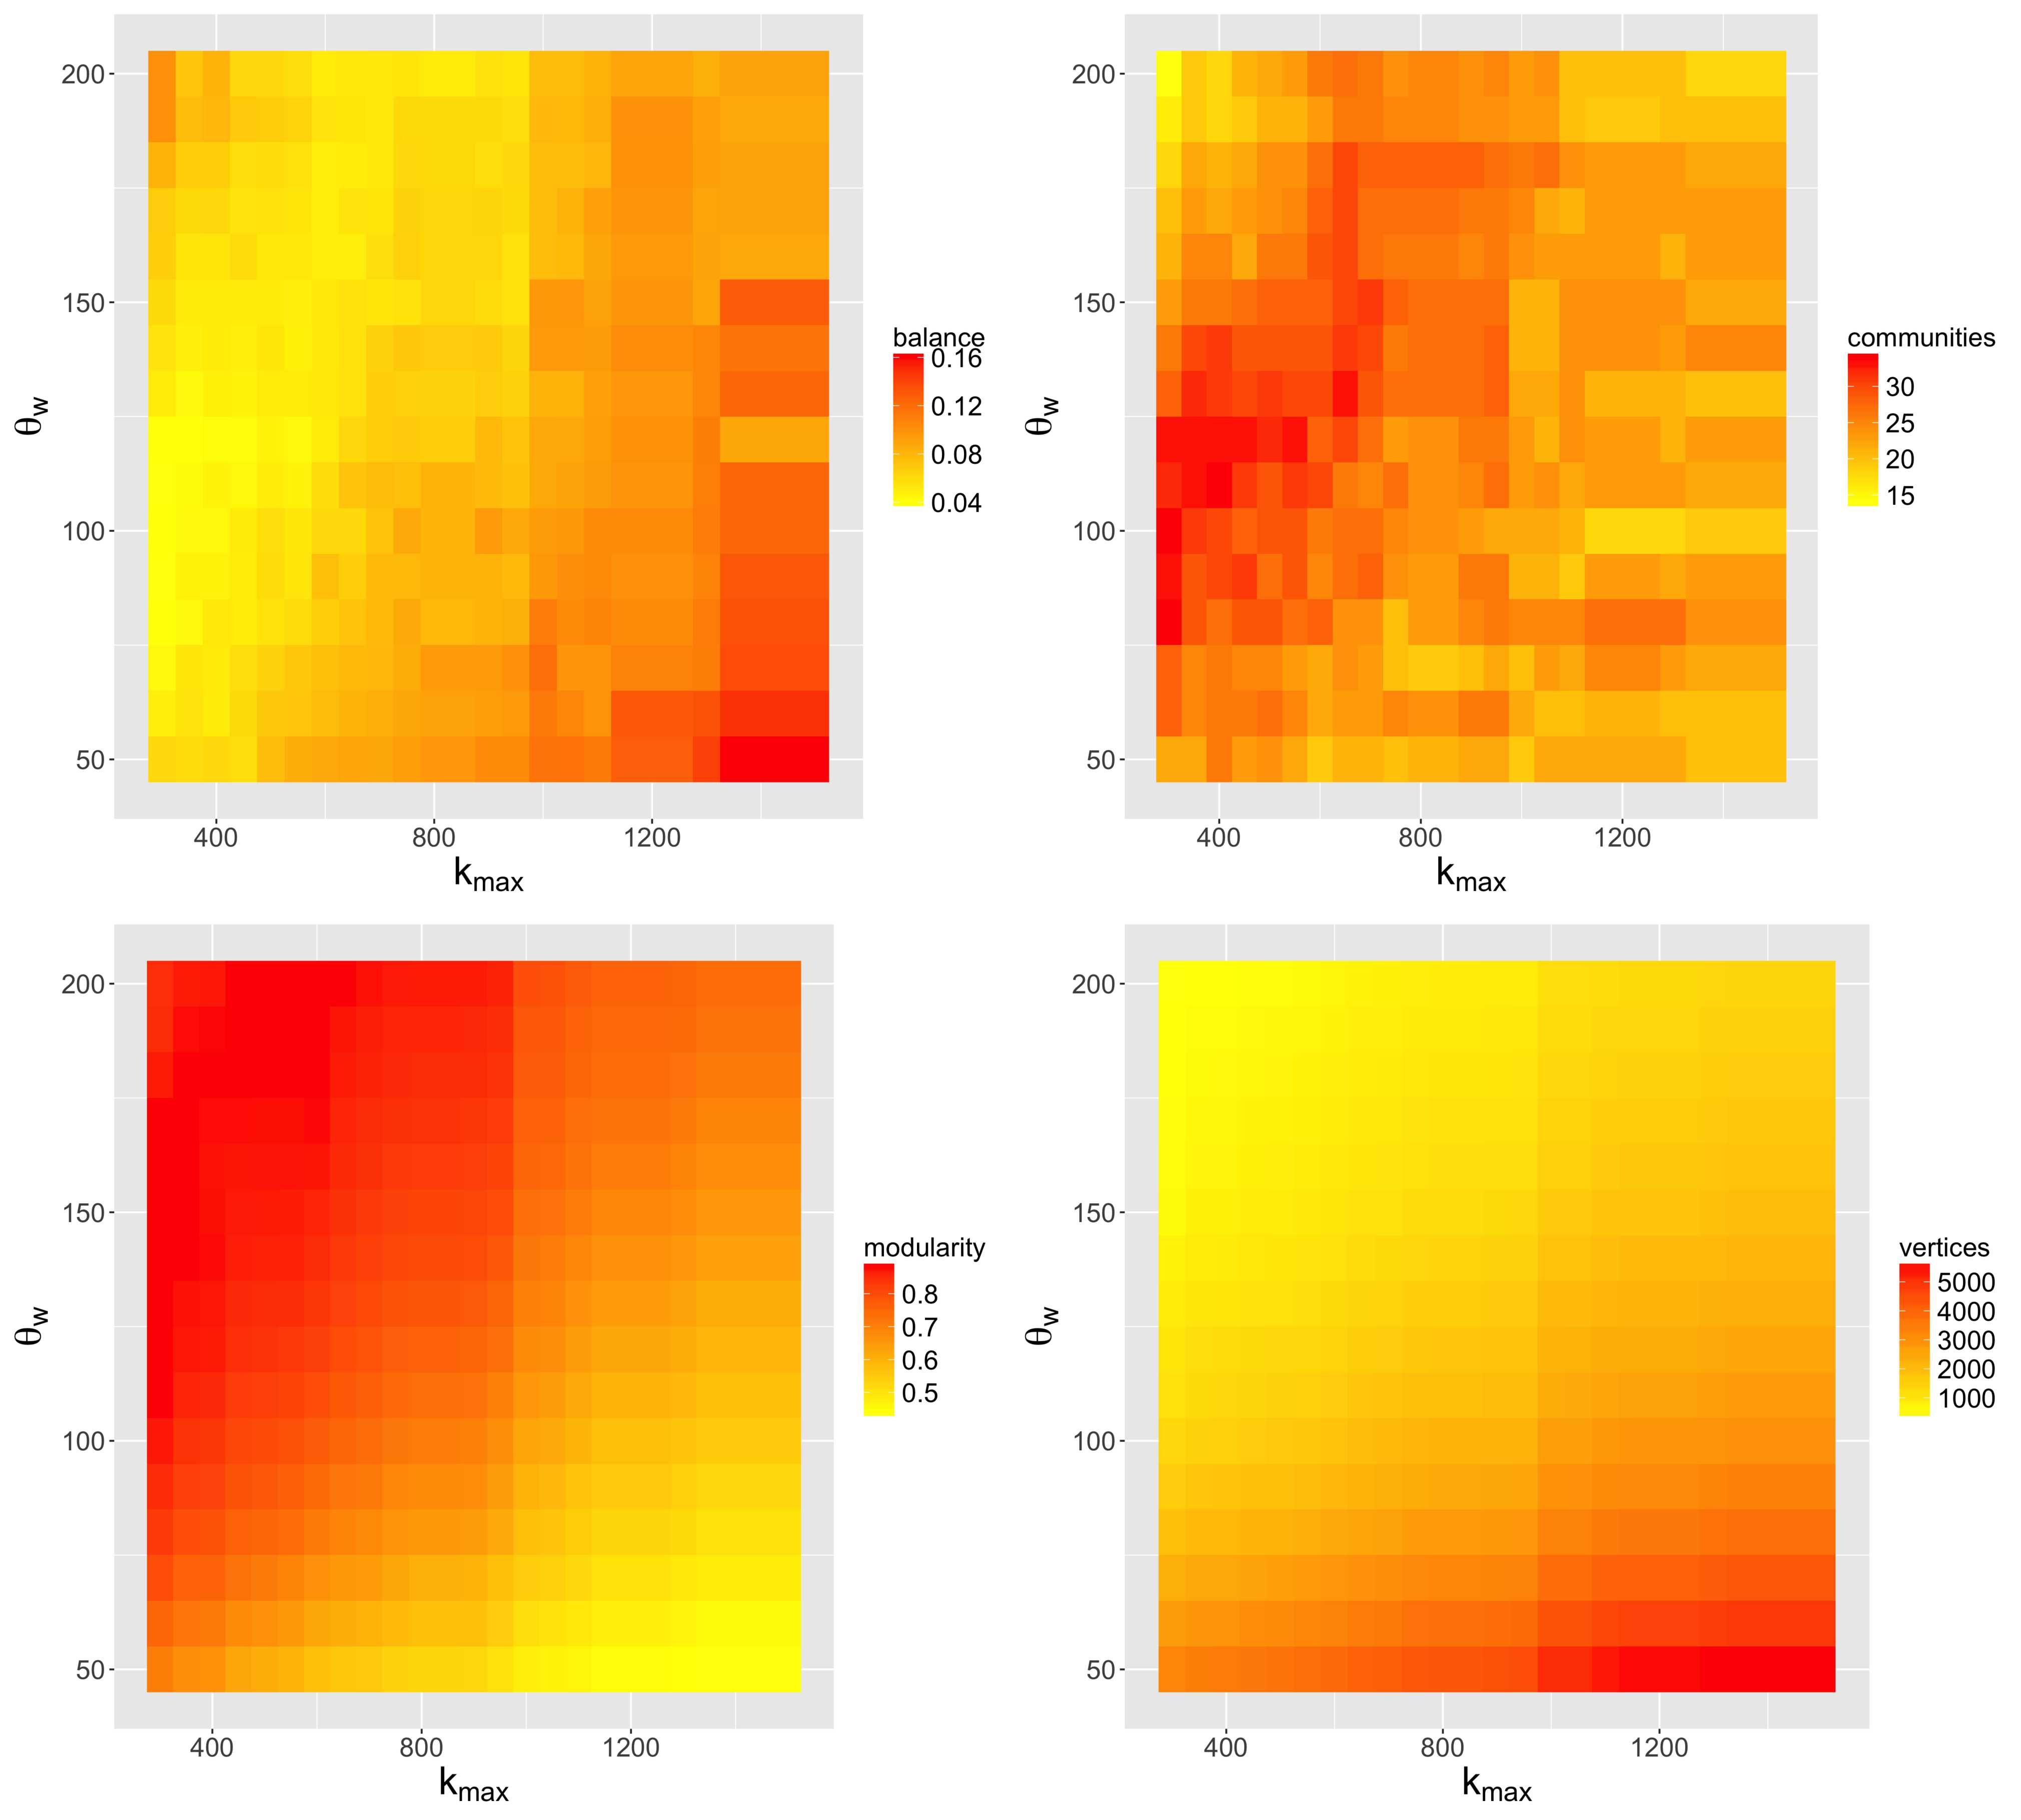
\includegraphics[width=\textwidth]{Figures/Cybergeo/Fig6.jpg}
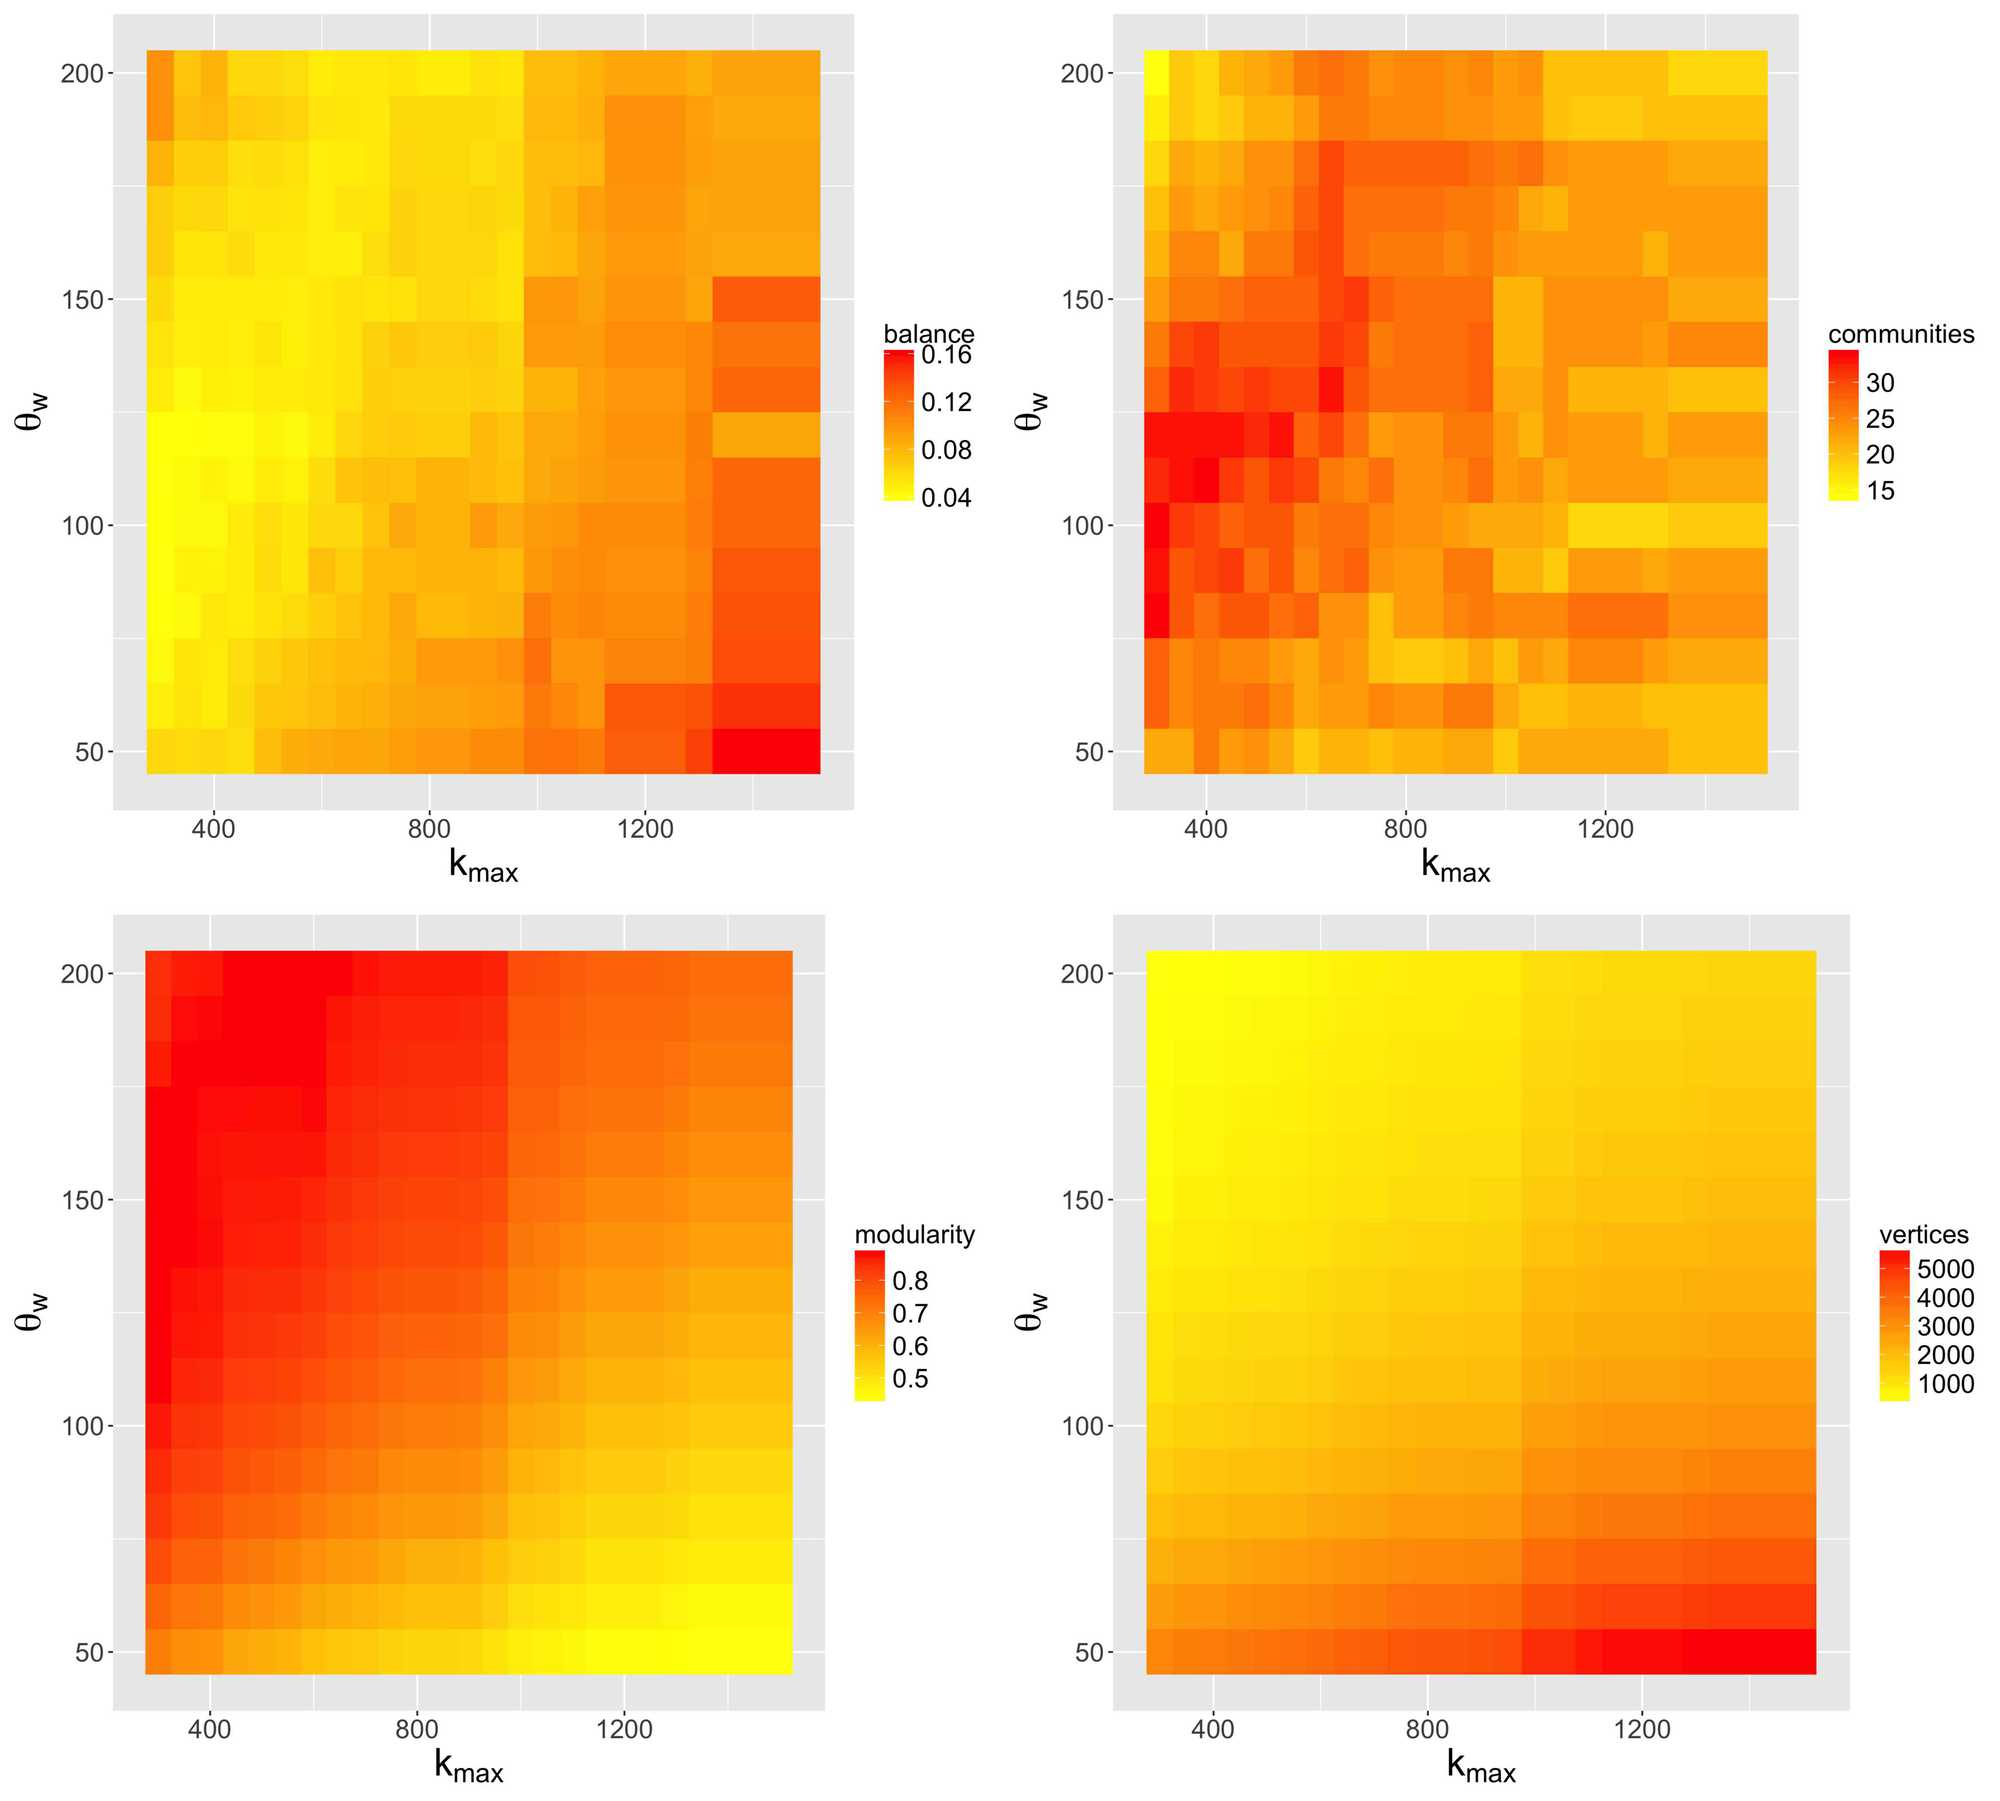
\includegraphics[width=\linewidth]{Figures/Final/B-cybergeo-fig6.jpg}
\caption{\textbf{Sensitivity analysis of network indicators to filtering parameters.} We show here 4 indicators (balance between community sizes, modularity of the decomposition, number of communities, number of vertices), as a function of parameters $k_{max}$ and $\theta_w$, at fixed $f_{min} = 50, f_{max} = 10000$. Close values for these two last parameters (in a reasonable range) give similar behavior.\label{fig:cybergeo:fig6}}{\textbf{Analyse de sensibilité des indicateurs de réseau aux paramètres de filtrage.}\label{fig:cybergeo:fig6}}
\end{figure}
%%%%%%%%%%%%%%%%%%





%%%%%%%%%%%%%%%%%%
\paragraph{Semantic Communities}{Communautés sémantiques}

We obtain therein communities in the semantic network with the optimized filtering parameters. At the exception of a small proportion apparently resulting from noise (representing less than 10 keywords in 3 communities that we remove, i.e. 0.33\% of keywords), communities correspond to well-defined scientific fields, domains, or approaches. Naming is also done by inspection of the most relevant keywords in each community, in order to stick here to a certain level of supervision.



%%%%%%%%%%%%%%%%%%
\begin{table}
\caption{\textbf{Semantic communities reconstructed from community detection in the semantic network.}\label{tab:cybergeo:domains}}{\textbf{Composition des communautés sémantiques.}\label{tab:cybergeo:domains}}
%\hspace{-2cm}
\begin{tabular}{lll}
\hline\noalign{\smallskip}
Name & Size & Keywords  \\
\noalign{\smallskip}\hline\noalign{\smallskip}
Political sciences/critical geography & 535 & \texttt{decision-mak, polit ideolog, democraci, stakehold, neoliber} \\
Biogeography & 394 & \texttt{plant densiti, wood, wetland, riparian veget} \\
Economic geography & 343 &  \texttt{popul growth, transact cost, socio-econom, household incom} \\
Environnment/climate & 309 & \texttt{ice sheet, stratospher, air pollut, climat model} \\
Complex systems & 283 & \texttt{scale-fre, multifract, agent-bas model, self-organ} \\
Physical geography & 203 & \texttt{sedimentari, digit elev model, geolog, river delta} \\
Spatial analysis & 175 & \texttt{spatial analysi, princip compon analysi, heteroscedast, factor analysi} \\
Microbiology & 118 & \texttt{chromosom, phylogenet, borrelia} \\
Statistical methods & 88 & \texttt{logist regress, classifi, kalman filter, sampl size} \\
Cognitive sciences & 81 & \texttt{semant memori, retrospect, neuroimag} \\
GIS & 75 & \texttt{geograph inform scienc, softwar design, volunt geograph inform, spatial decis support} \\
Traffic modeling & 63 & \texttt{simul model, lane chang, traffic flow, crowd behavior} \\
Health & 52 & \texttt{epidem, vaccin strategi, acut respiratori syndrom, hospit} \\
Remote sensing & 48 & \texttt{land-cov, landsat imag, lulc} \\
Crime & 17 & \texttt{crimin justic system, social disorgan, crime} \\
\noalign{\smallskip}\hline
\end{tabular}
\end{table}
%%%%%%%%%%%%%%%%%%


%%%%%%%%%%%%%%%%%%
\begin{figure}
%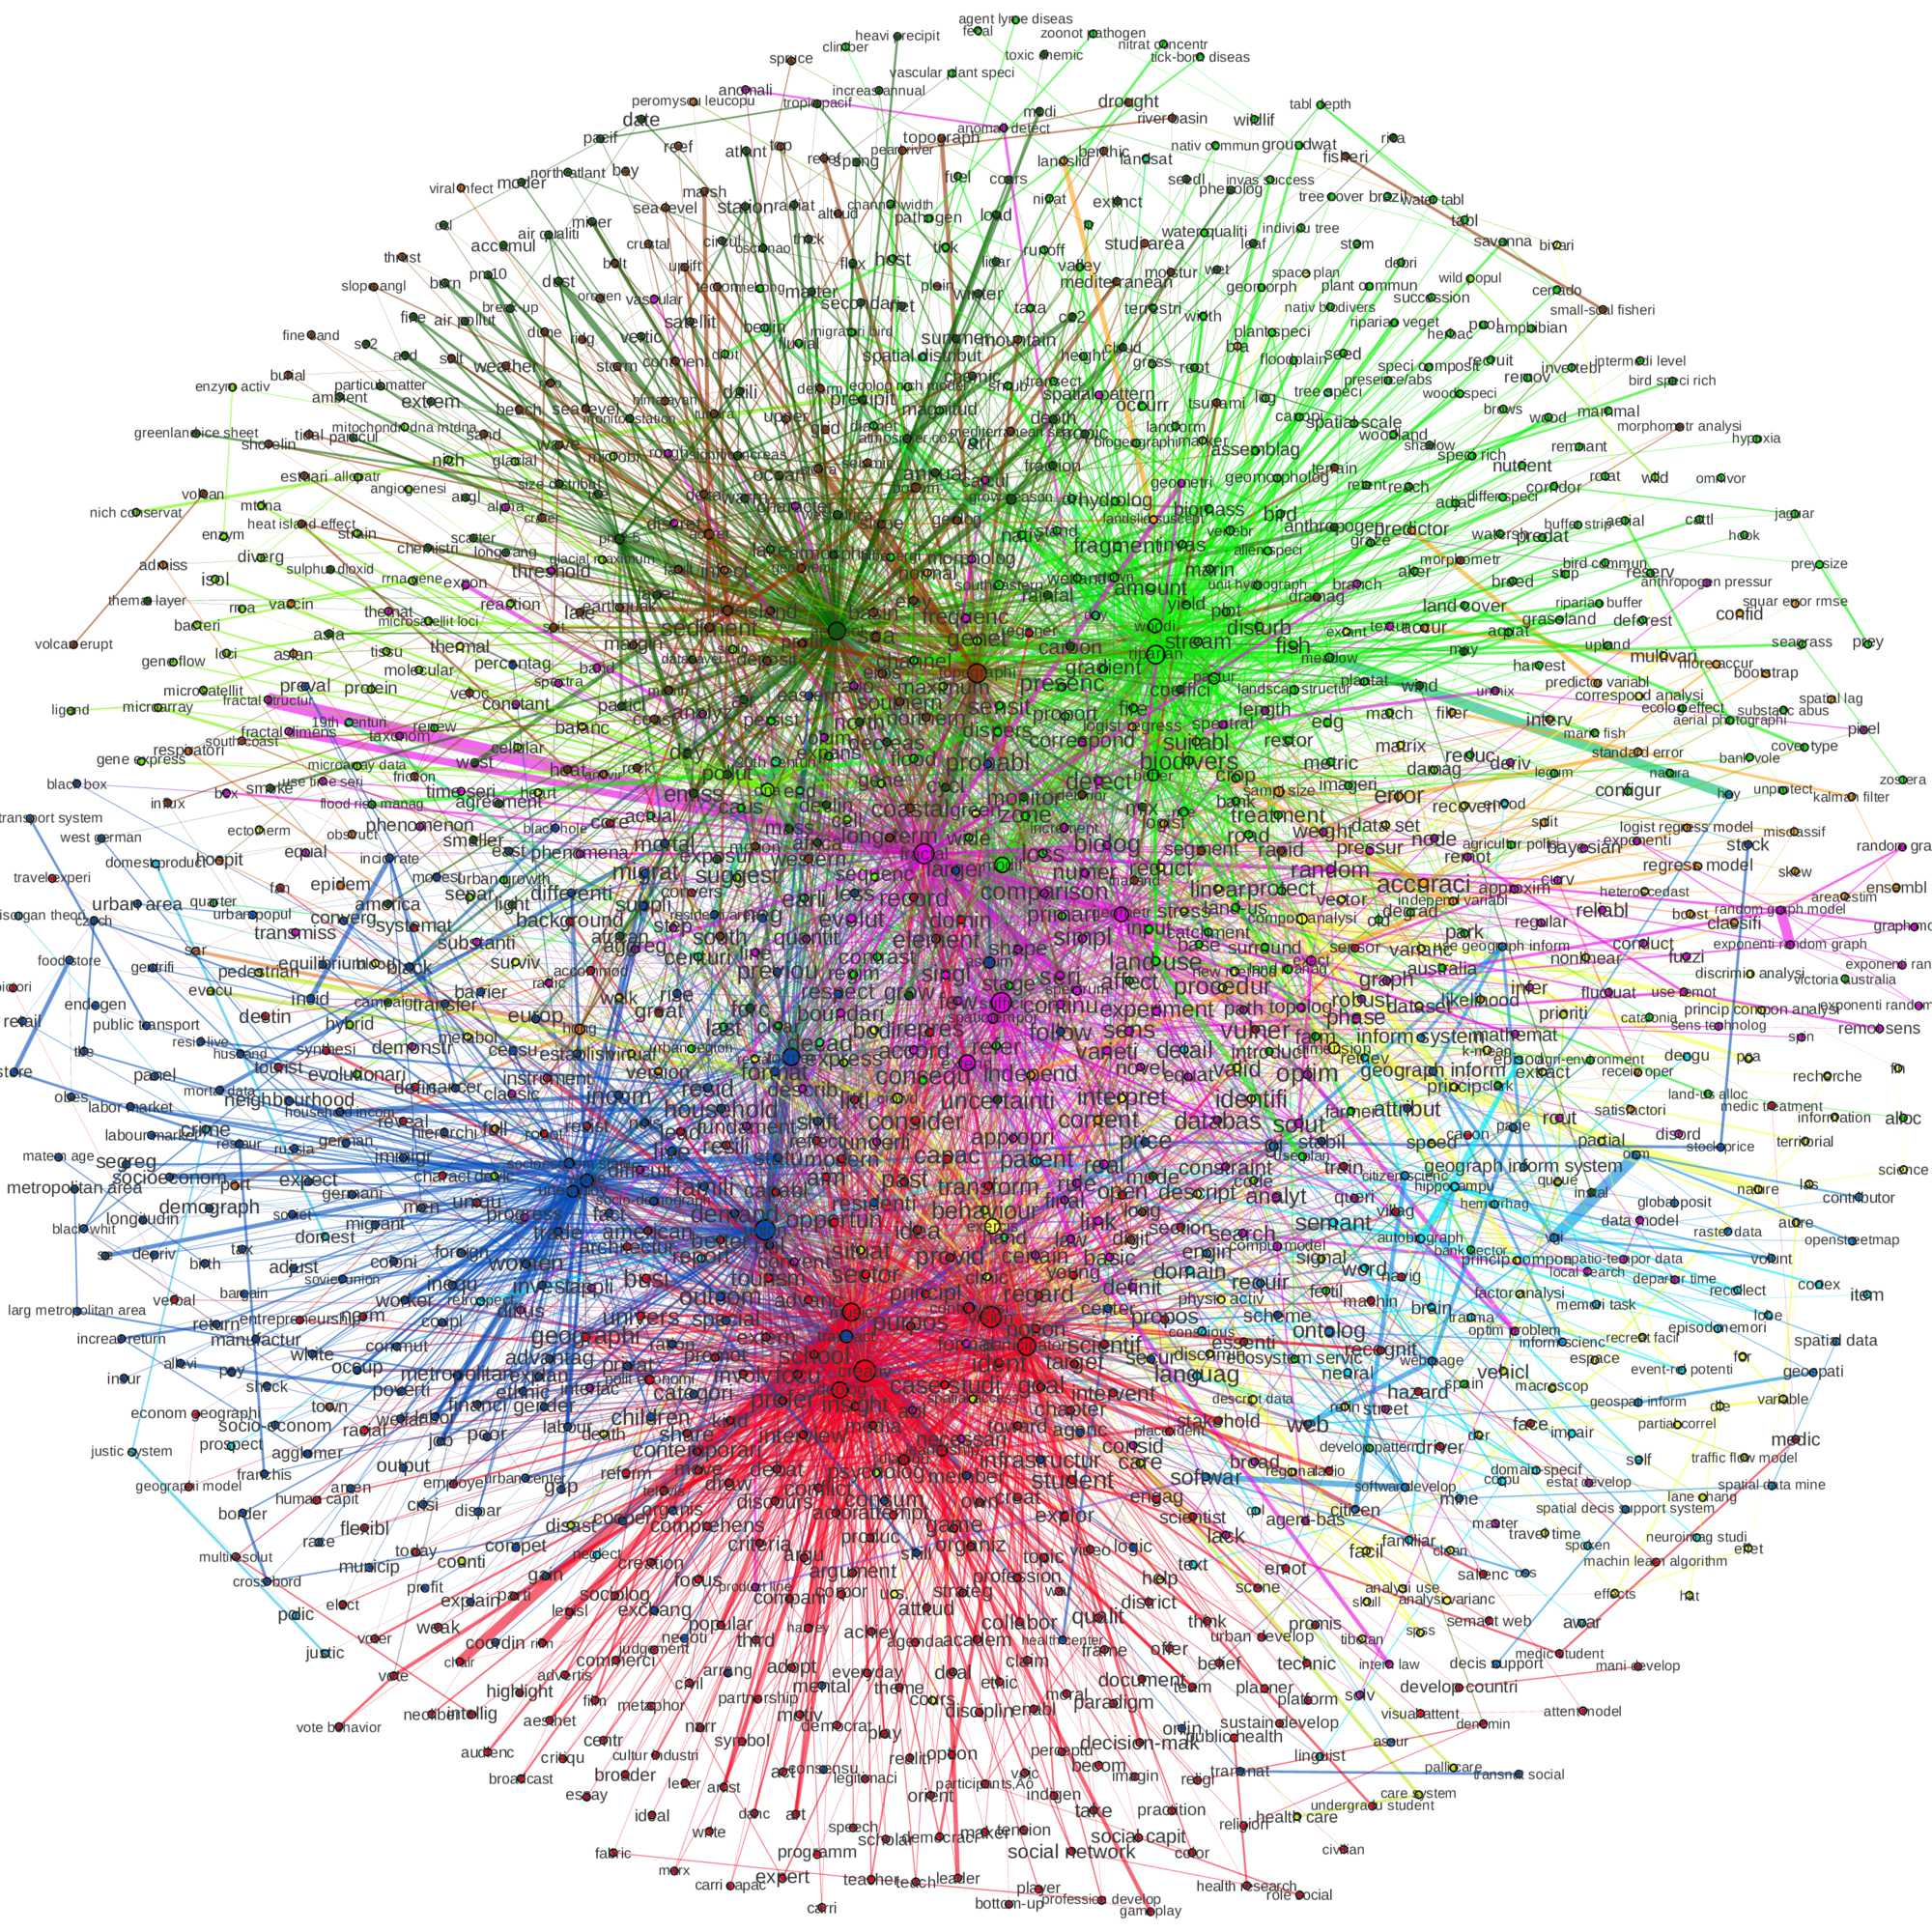
\includegraphics[width=1.6\textwidth]{Figures/Cybergeo/Fig7.jpg}
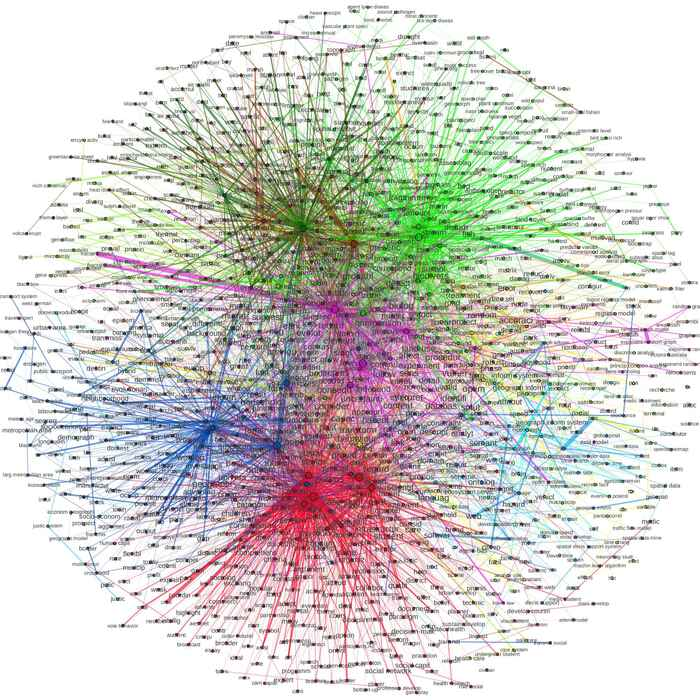
\includegraphics[width=\linewidth]{Figures/Cybergeo/B-cybergeo-fig7.jpg}
\caption{\textbf{Visualization of the semantic network.} Network is constructed by co-occurrences of most relevant keywords. Filtering parameters are here taken according to the multi-objective optimization done in Fig.~\ref{fig:sensitivity}, i.e. $(k_{max}=1200,\theta_w=100,f_{min}=50,f_{max}=10000)$. The graph spatialization algorithm (Fruchterman-Reingold), despite its stochastic and path-dependent character, unveils information on the relative positioning of communities.\label{fig:cybergeo:fig7}}{\textbf{Visualisation du réseau sémantique.}\label{fig:cybergeo:fig7}}
\end{figure}
%%%%%%%%%%%%%%%%%%



%%%%%%%%%%%%%%%%%%
\begin{figure}
%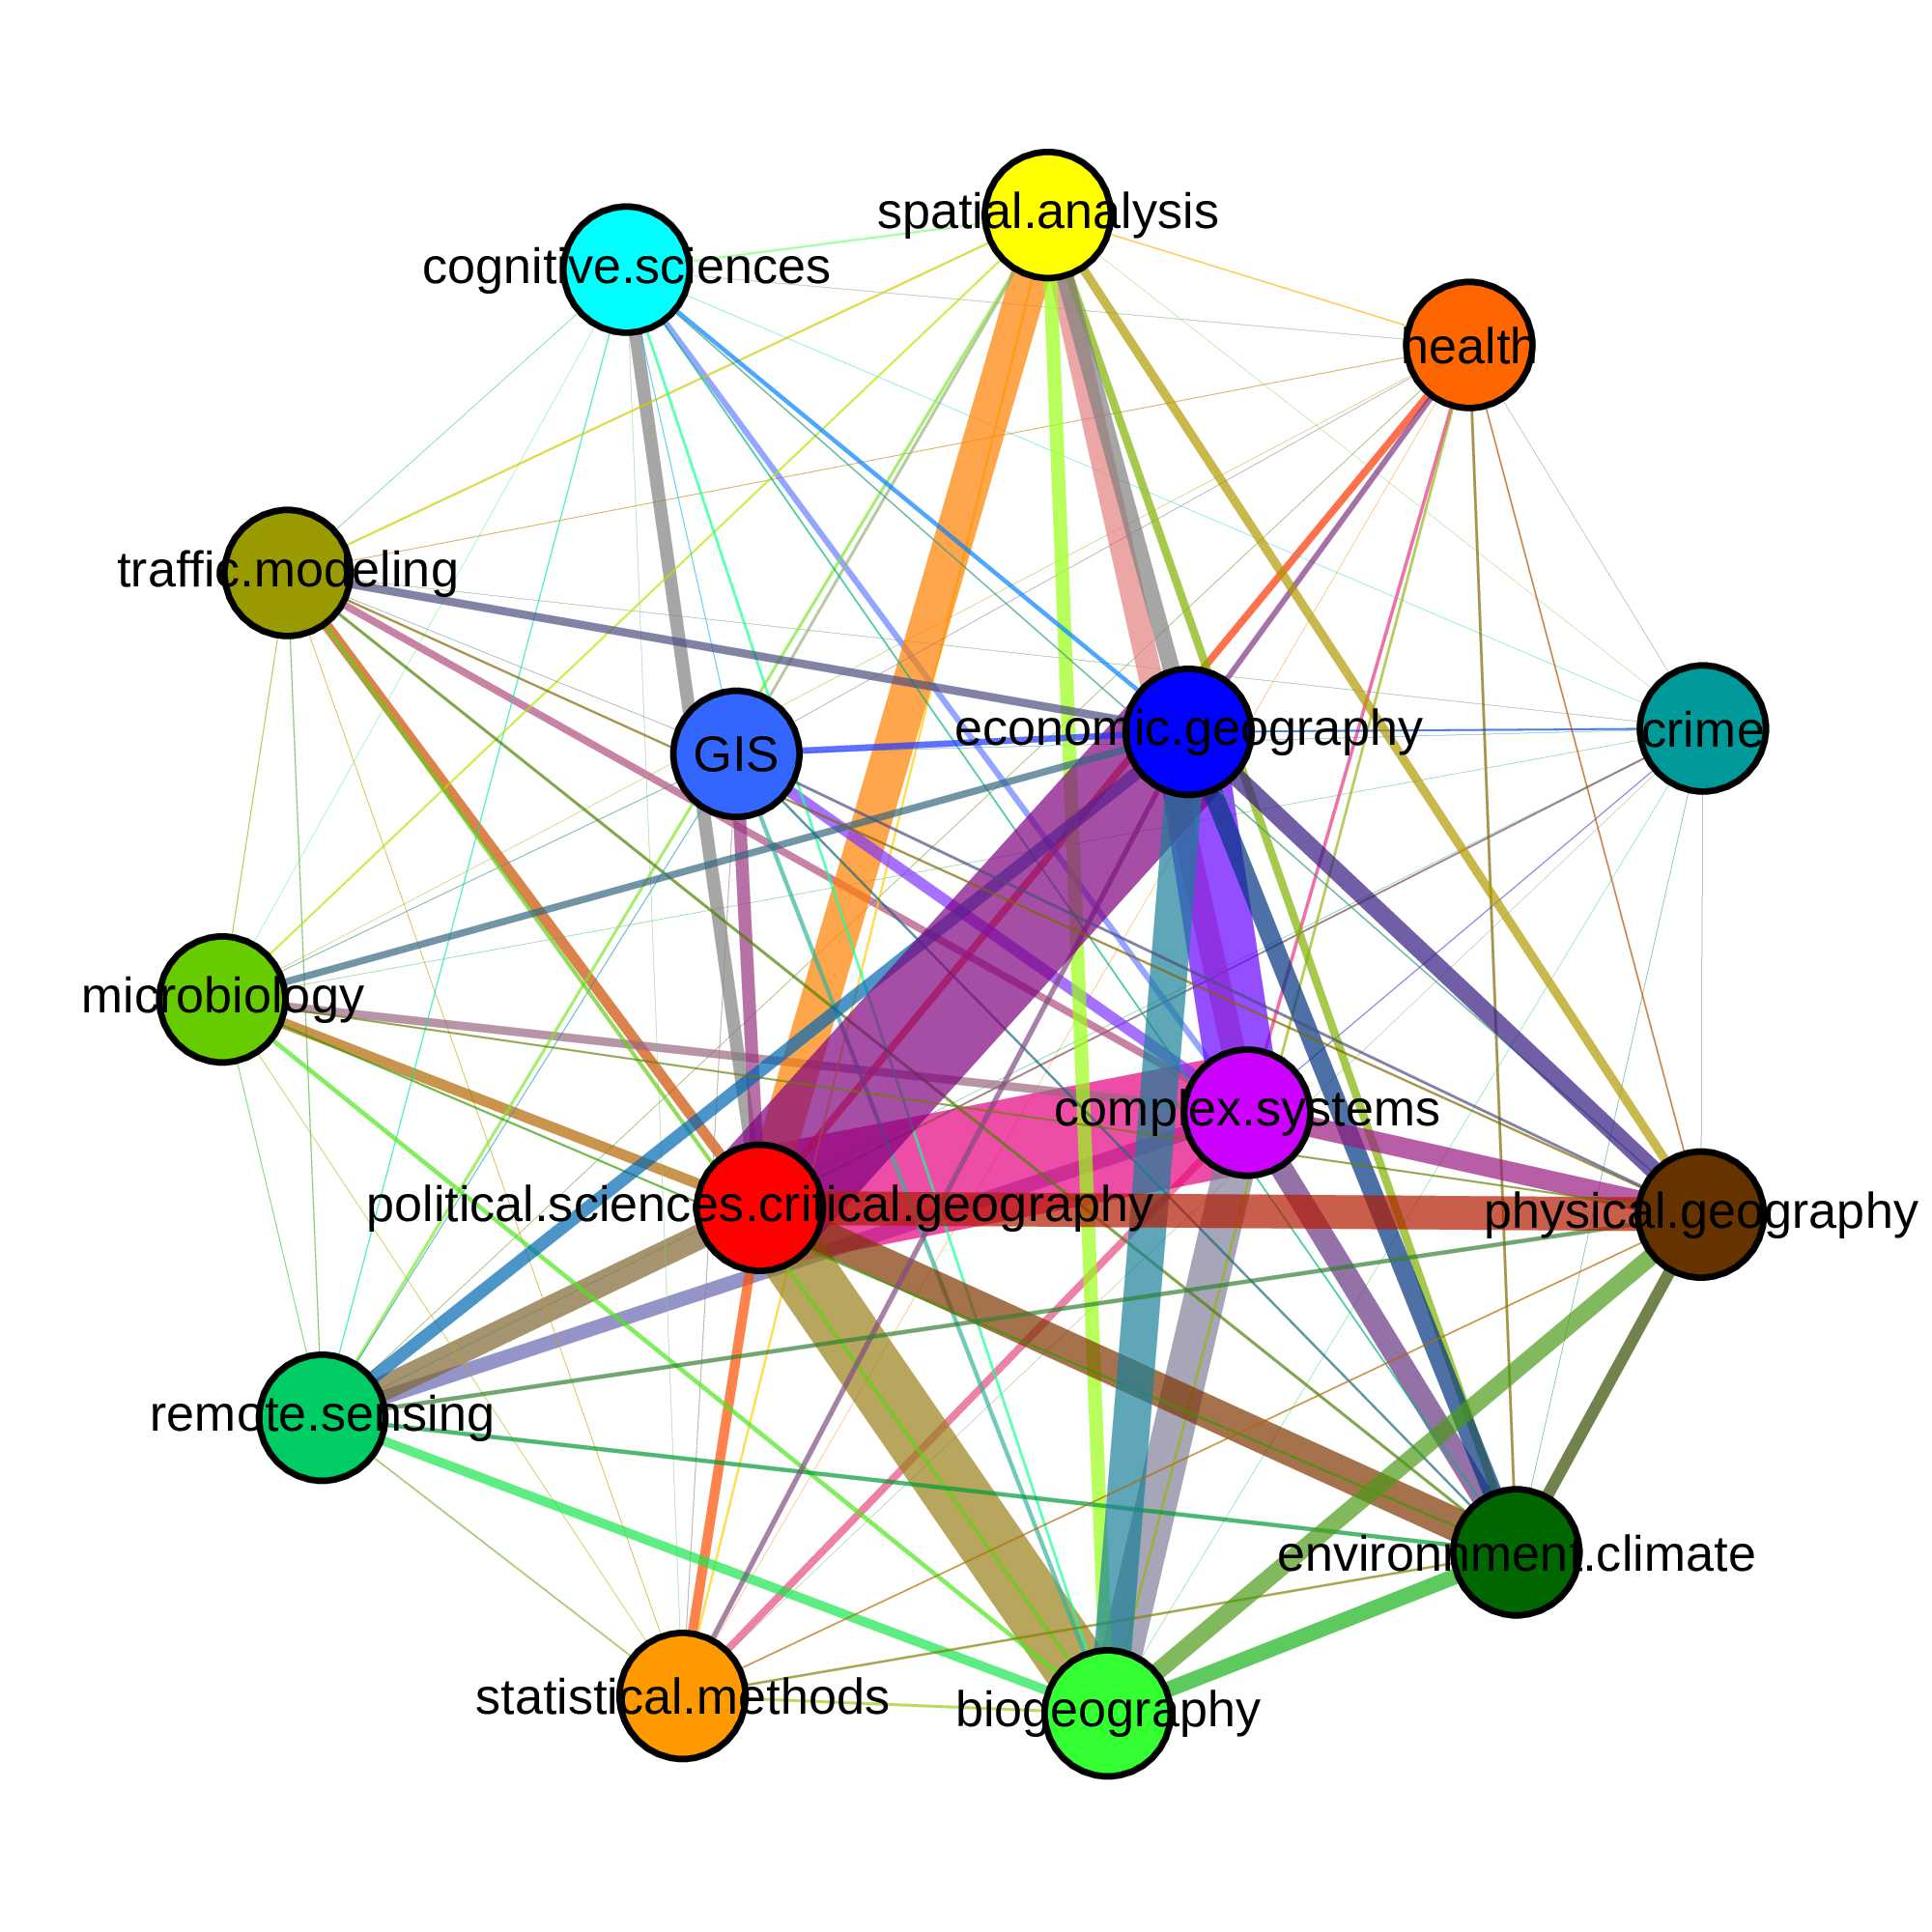
\includegraphics[width=\textwidth]{Figures/Cybergeo/Fig8.jpg}
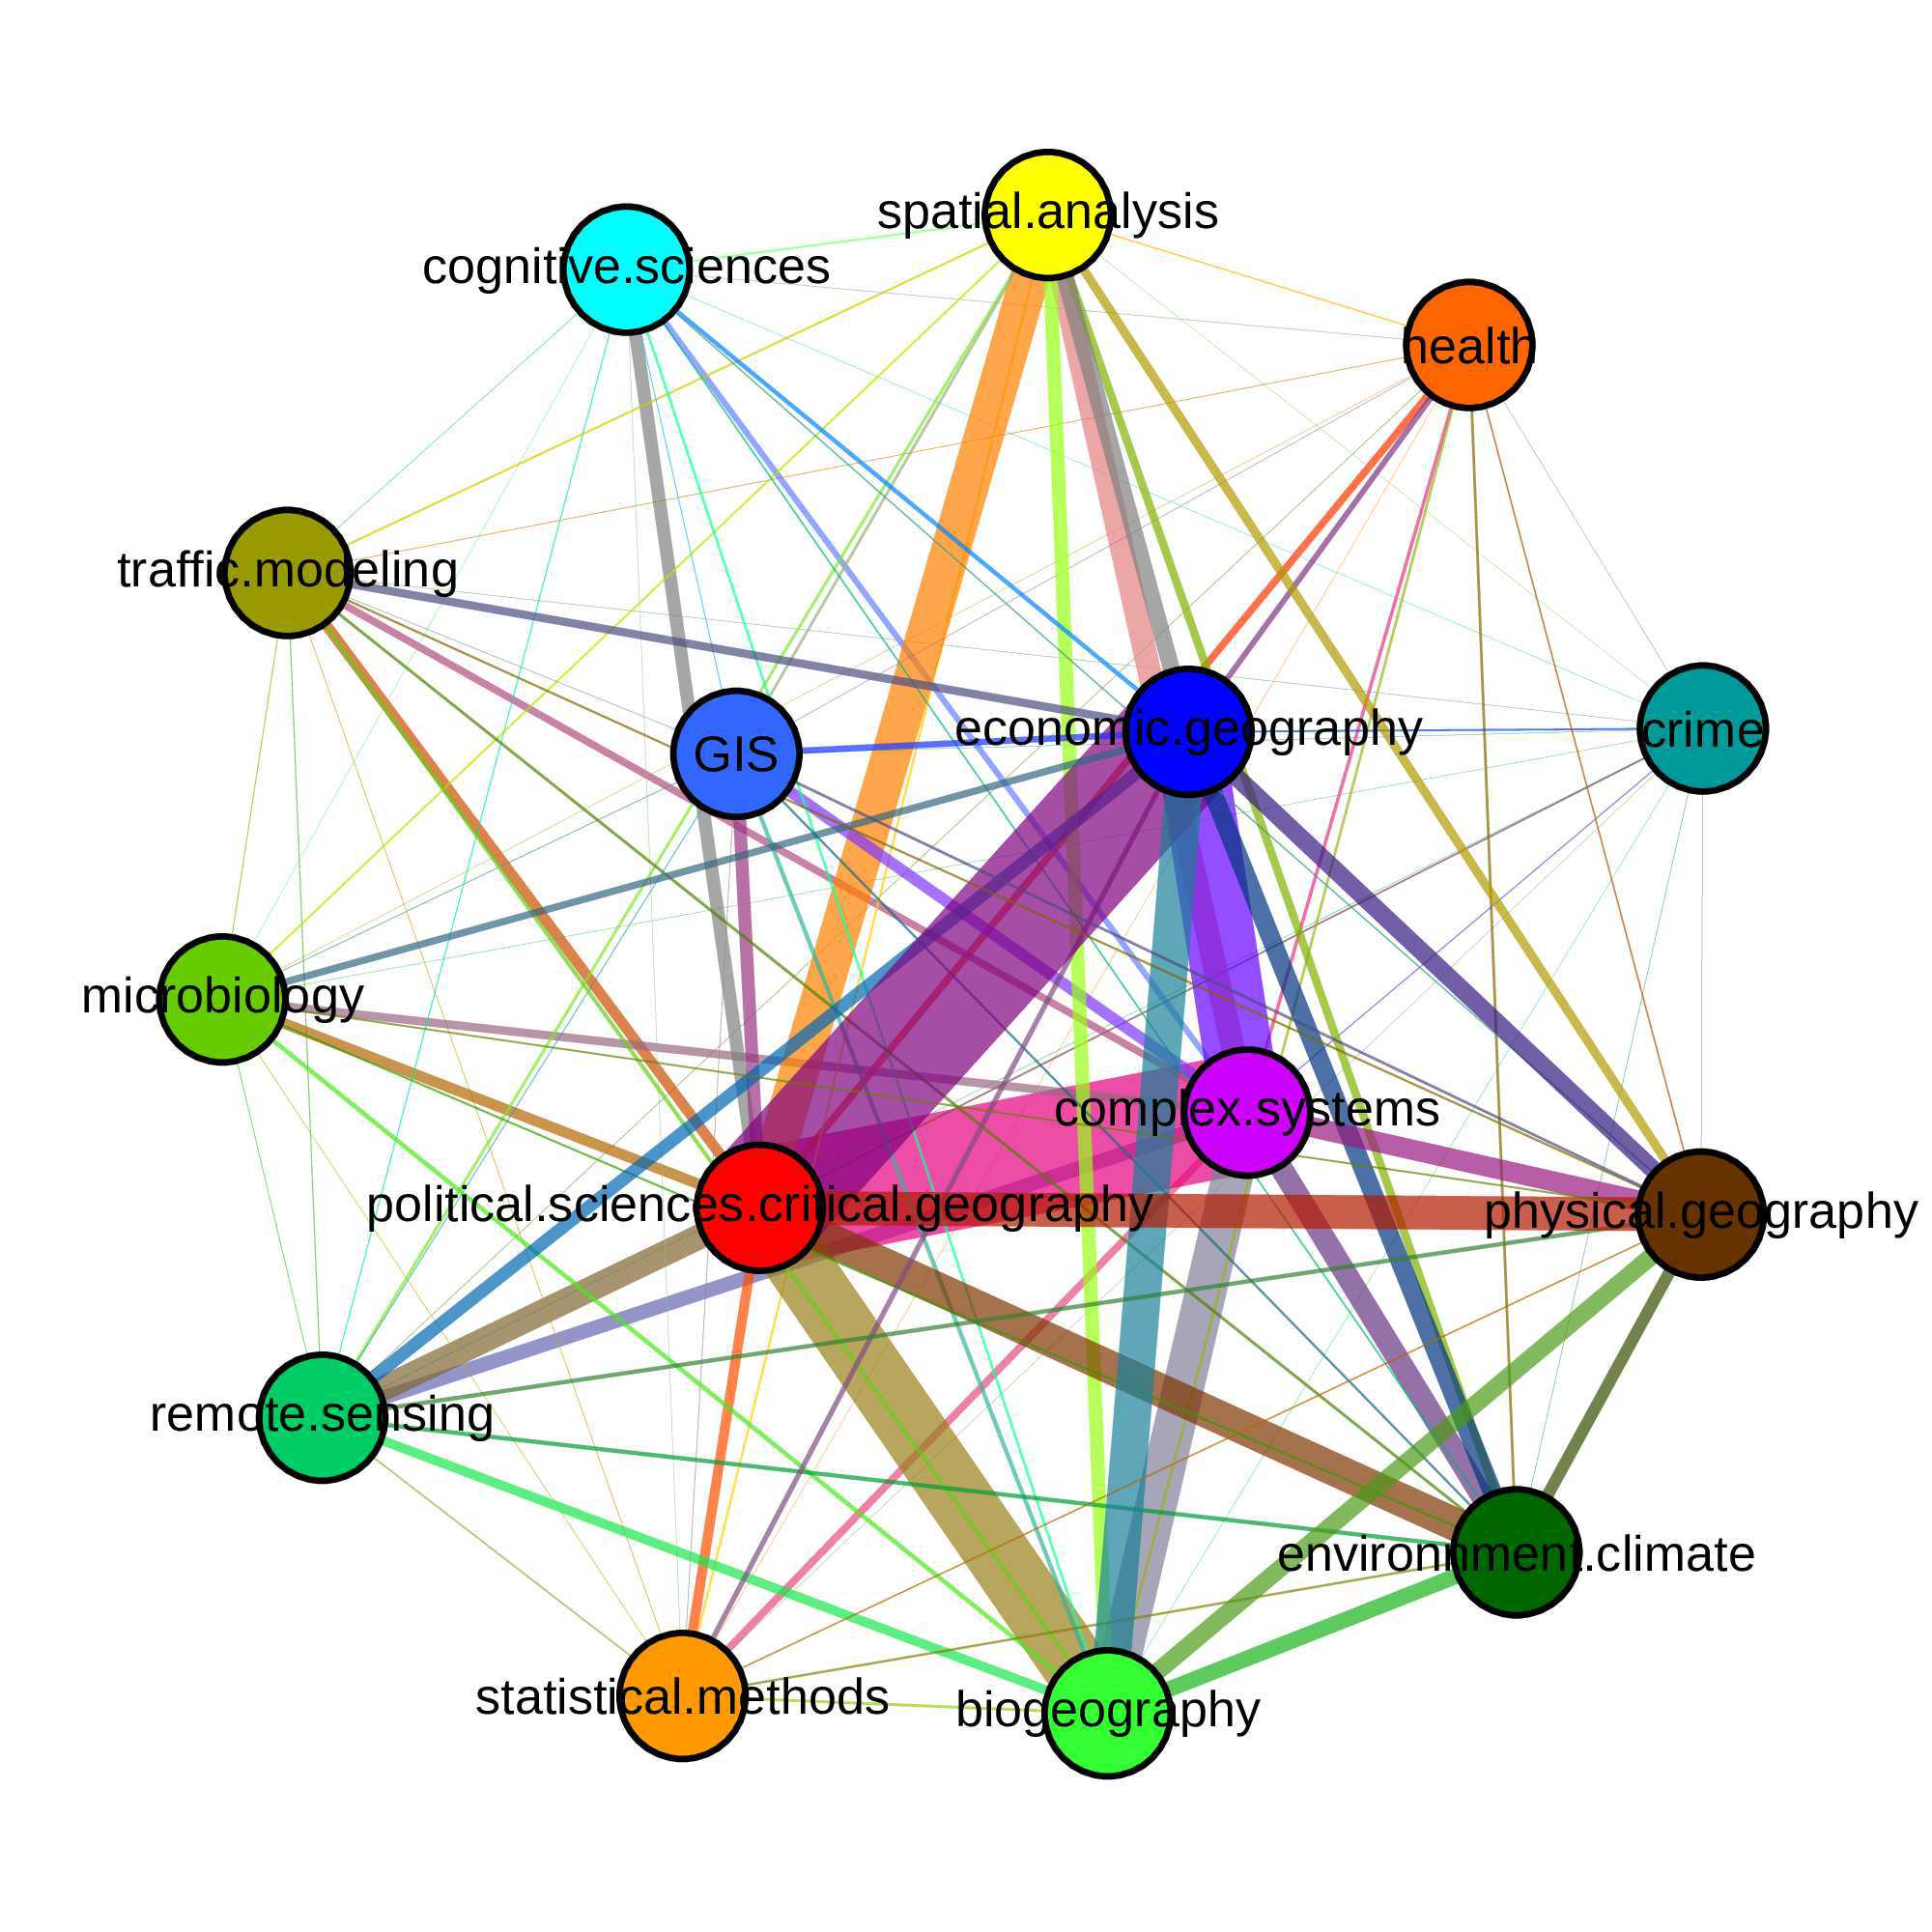
\includegraphics[width=\textwidth]{Figures/Final/B-cybergeo-fig8.jpg}
\caption{\textbf{Synthesis of semantic communities and their links.} Weights of links are computed as probabilities of co-occurrences of corresponding keywords within references.\label{fig:cybergeo:fig8}}{\textbf{Synthèse des communautés sémantiques et de leurs liens.}\label{fig:cybergeo:fig8}}
\end{figure}
%%%%%%%%%%%%%%%%%%

Table~\ref{tab:cybergeo:domains} summarizes the communities, giving their names, sizes, and corresponding keywords. The most important community is related to issues in political science and critical geography, what could have been expected as several previously obtained citations communities (Social geography, Urban studies) deal with these issues. We then obtain a large cluster of terms related to biogeography, that must correspond to publications in Ecology and Socio-ecology identified before, together with a community in Environment and Climate.


In a way similar to the citation communities, but more pronounced here, we obtain endogenous ``disciplines'' that can correspond to real disciplines, to methodologies, to object of studies. This classification thus also unveil \emph{effective scientific practices}, here in terms of semantic content. A class here related to complex systems can be associated to a paradigm and various approaches that were separated in the citation communities : agent-based models and complex networks for example. On the contrary, some studies that were gathered in a large domain before can be precisely differentiated in the semantic network, such as microbiology and health here that are used by studies related to socio-ecology or ecology in the citation network. Some very specific domains appear here as they have very few connections in their actual semantic content : for example, Geography of crime is very precise and disconnected from other communities.


We show in Fig.~\ref{fig:cybergeo:fig7} a visualisation of the semantic network, in which the positioning of communities, induced by a Fruchterman-Reingold algorithm (that we use here to have a more precise layout in the relative positioning compared to Force Atlas~\citep{jacomy2014forceatlas2}). The bridging between distant disciplines is done quite differently compared to the citation network, and reveals thus qualitatively an other dimension of interdisciplinarity, i.e. the semantics shared by disciplines. Here, the communities corresponding to Economic Geography (blue) and to Critical Geography (red) are close as in the citation network, but are linked to ecology and geomorphology (green and brown) by Complex Systems (magenta), although these were not present as a community in the citation network. Complexity methodologies such as Fractals, Scaling~\citep{west2017scale} or Networks~\citep{newman2003structure} are indeed widely used both in social sciences and in physics or biology. The semantic analysis reveals thus that very distant disciplines, that are distant in their citation patterns, are finally close in terms of actual content.



In terms of overlaps between communities, in the sense of co-occurrences of corresponding keywords within texts of references, we show a synthesis of links between semantic communities in Fig.~\ref{fig:cybergeo:fig8}. We see that communities such as Critical Geography and Biogeography are not totally disconnected and share still a certain number of co-occurrences. More isolated communities can be spotted such as Health and Crime Geographies. Surprisingly, Statistical Methods does not share strong links with other communities, what could mean that articles dealing with methodological issues in this field are rather disconnected from the field of application, or at least do not describe it extensively. On the contrary, methods in Complex Systems are organically integrated with the thematic issues they tackle.








%%%%%%%%%%%%%%%%%%
\subsubsection{Semantic composition of citation communities}{Composition sémantique des communautés de citation}


%%%%%%%%%%%%%%%%%%
\begin{figure}
%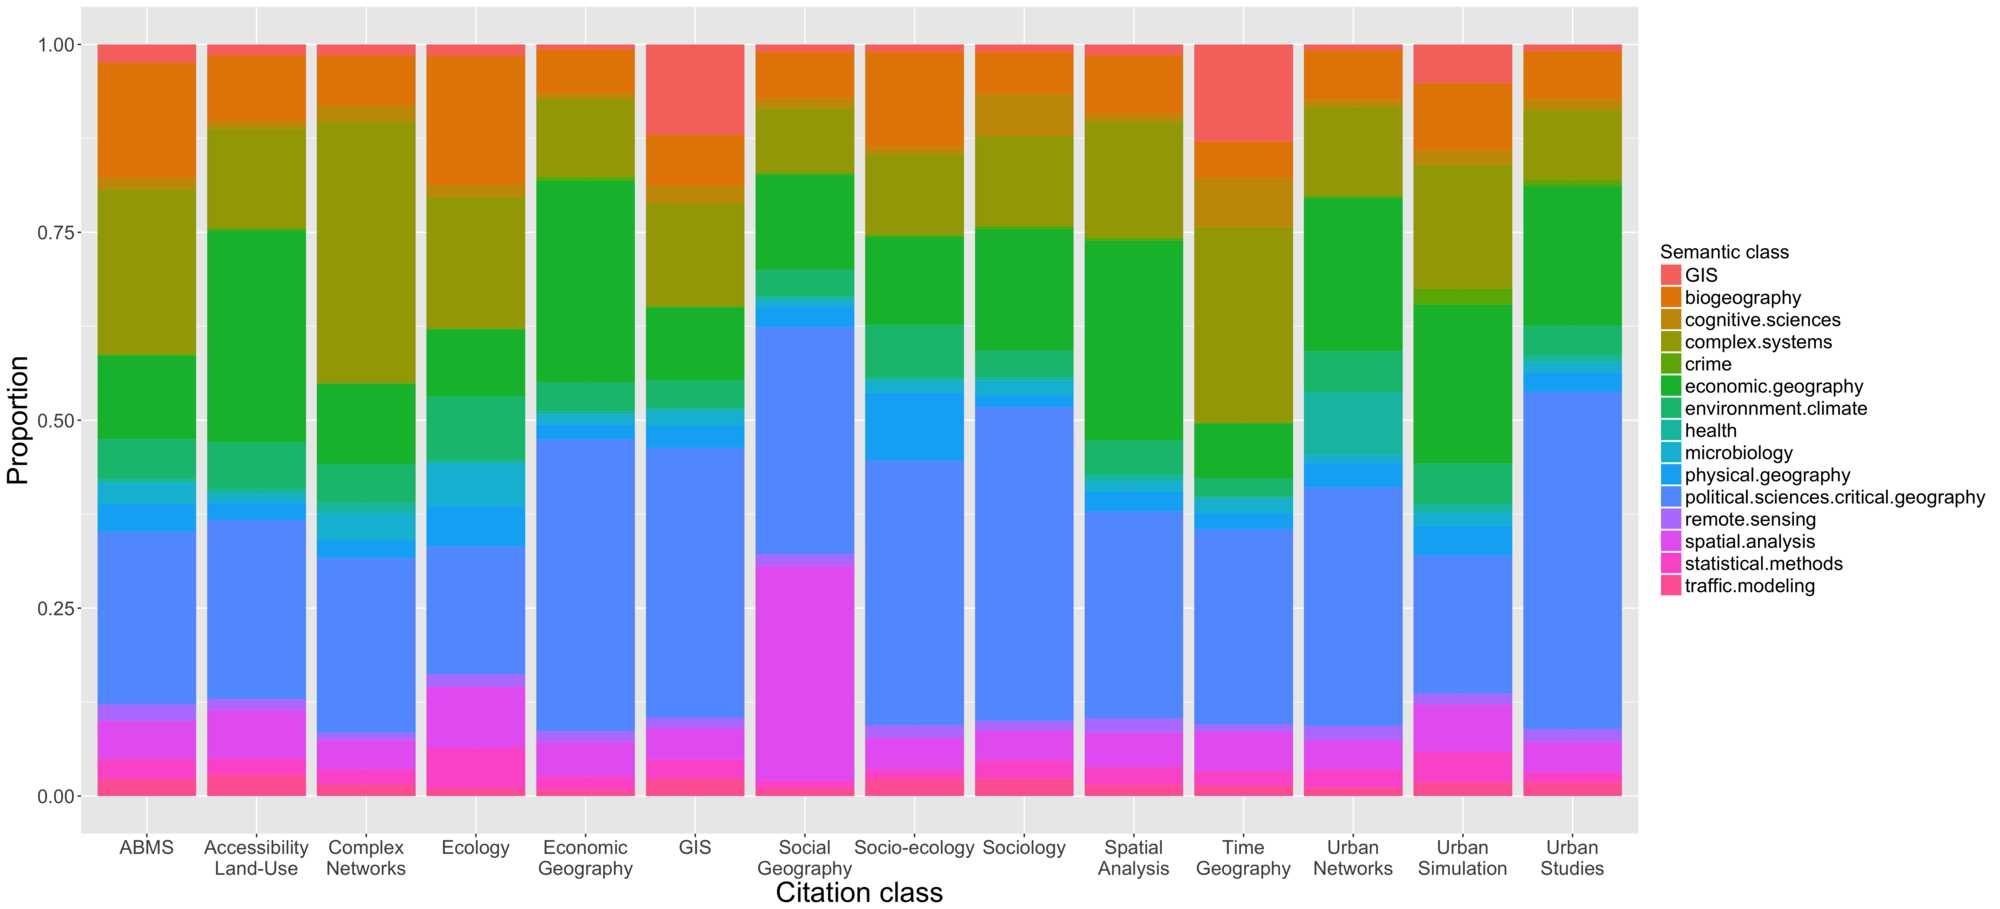
\includegraphics[width=\textwidth]{Figures/Cybergeo/Fig9.jpg}
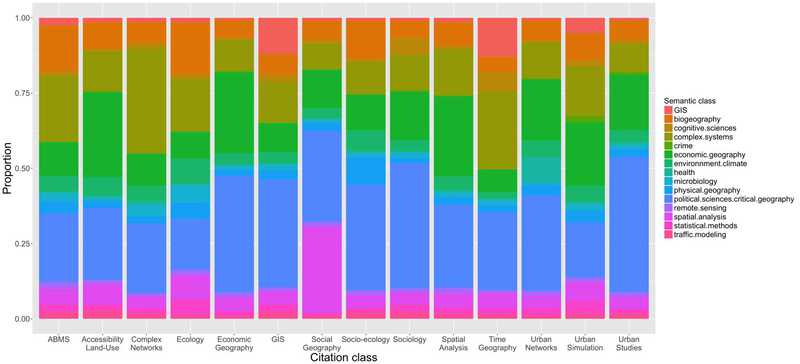
\includegraphics[width=\linewidth]{Figures/Final/B-cybergeo-fig9.jpg}
\caption{\textbf{Composition of citation communities in terms of semantic content.} For each citation class (horizontally), the bar is decomposed as the proportions of each semantic class (given by color).\label{fig:cybergeo:fig9}}{\textbf{Composition des communautés de citation en termes de contenu sémantique.}\label{fig:cybergeo:fig9}}
\end{figure}
%%%%%%%%%%%%%%%%%%


We can now turn to the study of the relation between classifications. First, a simple way to link them is to look at the semantic content of citation communities. Each reference has a given proportion of keywords within each semantic class, and an average composition in terms of semantic classes for each citation class can thus be computed. We show these composition in Fig.~\ref{fig:cybergeo:fig9}. Some expected results are obtained, such as Complex Networks (citation) having the largest part in Complex Systems (semantic), or GIS (citation) the largest in GIS (semantic), and similarly for Economic Geography.

But the study of patterns that could have not been expected is very informative, and unveils practices of interdisciplinarity. For example, Time Geography (citation) uses as much GIS (semantic) as GIS (citation), what means that they should be using the corresponding methods and tools to study the thematic question of spatio-temporal trajectories of geographical agents. The most important in terms of political science (semantic) are Urban Studies, what suggest a convergence of the City as an object of study and of the disciplines of Political Science and Critical Geography. Also interestingly, the citation communities using most biogeography are Ecology (what could have been expected) and ABMS, confirming again the role of the thematic application in complex systems methodologies.





%%%%%%%%%%%%%%%%%%
\subsubsection{Measuring interdisciplinarity}{Mesure de l'interdisciplinarité}


%%%%%%%%%%%%%%%%%%
\begin{figure}
%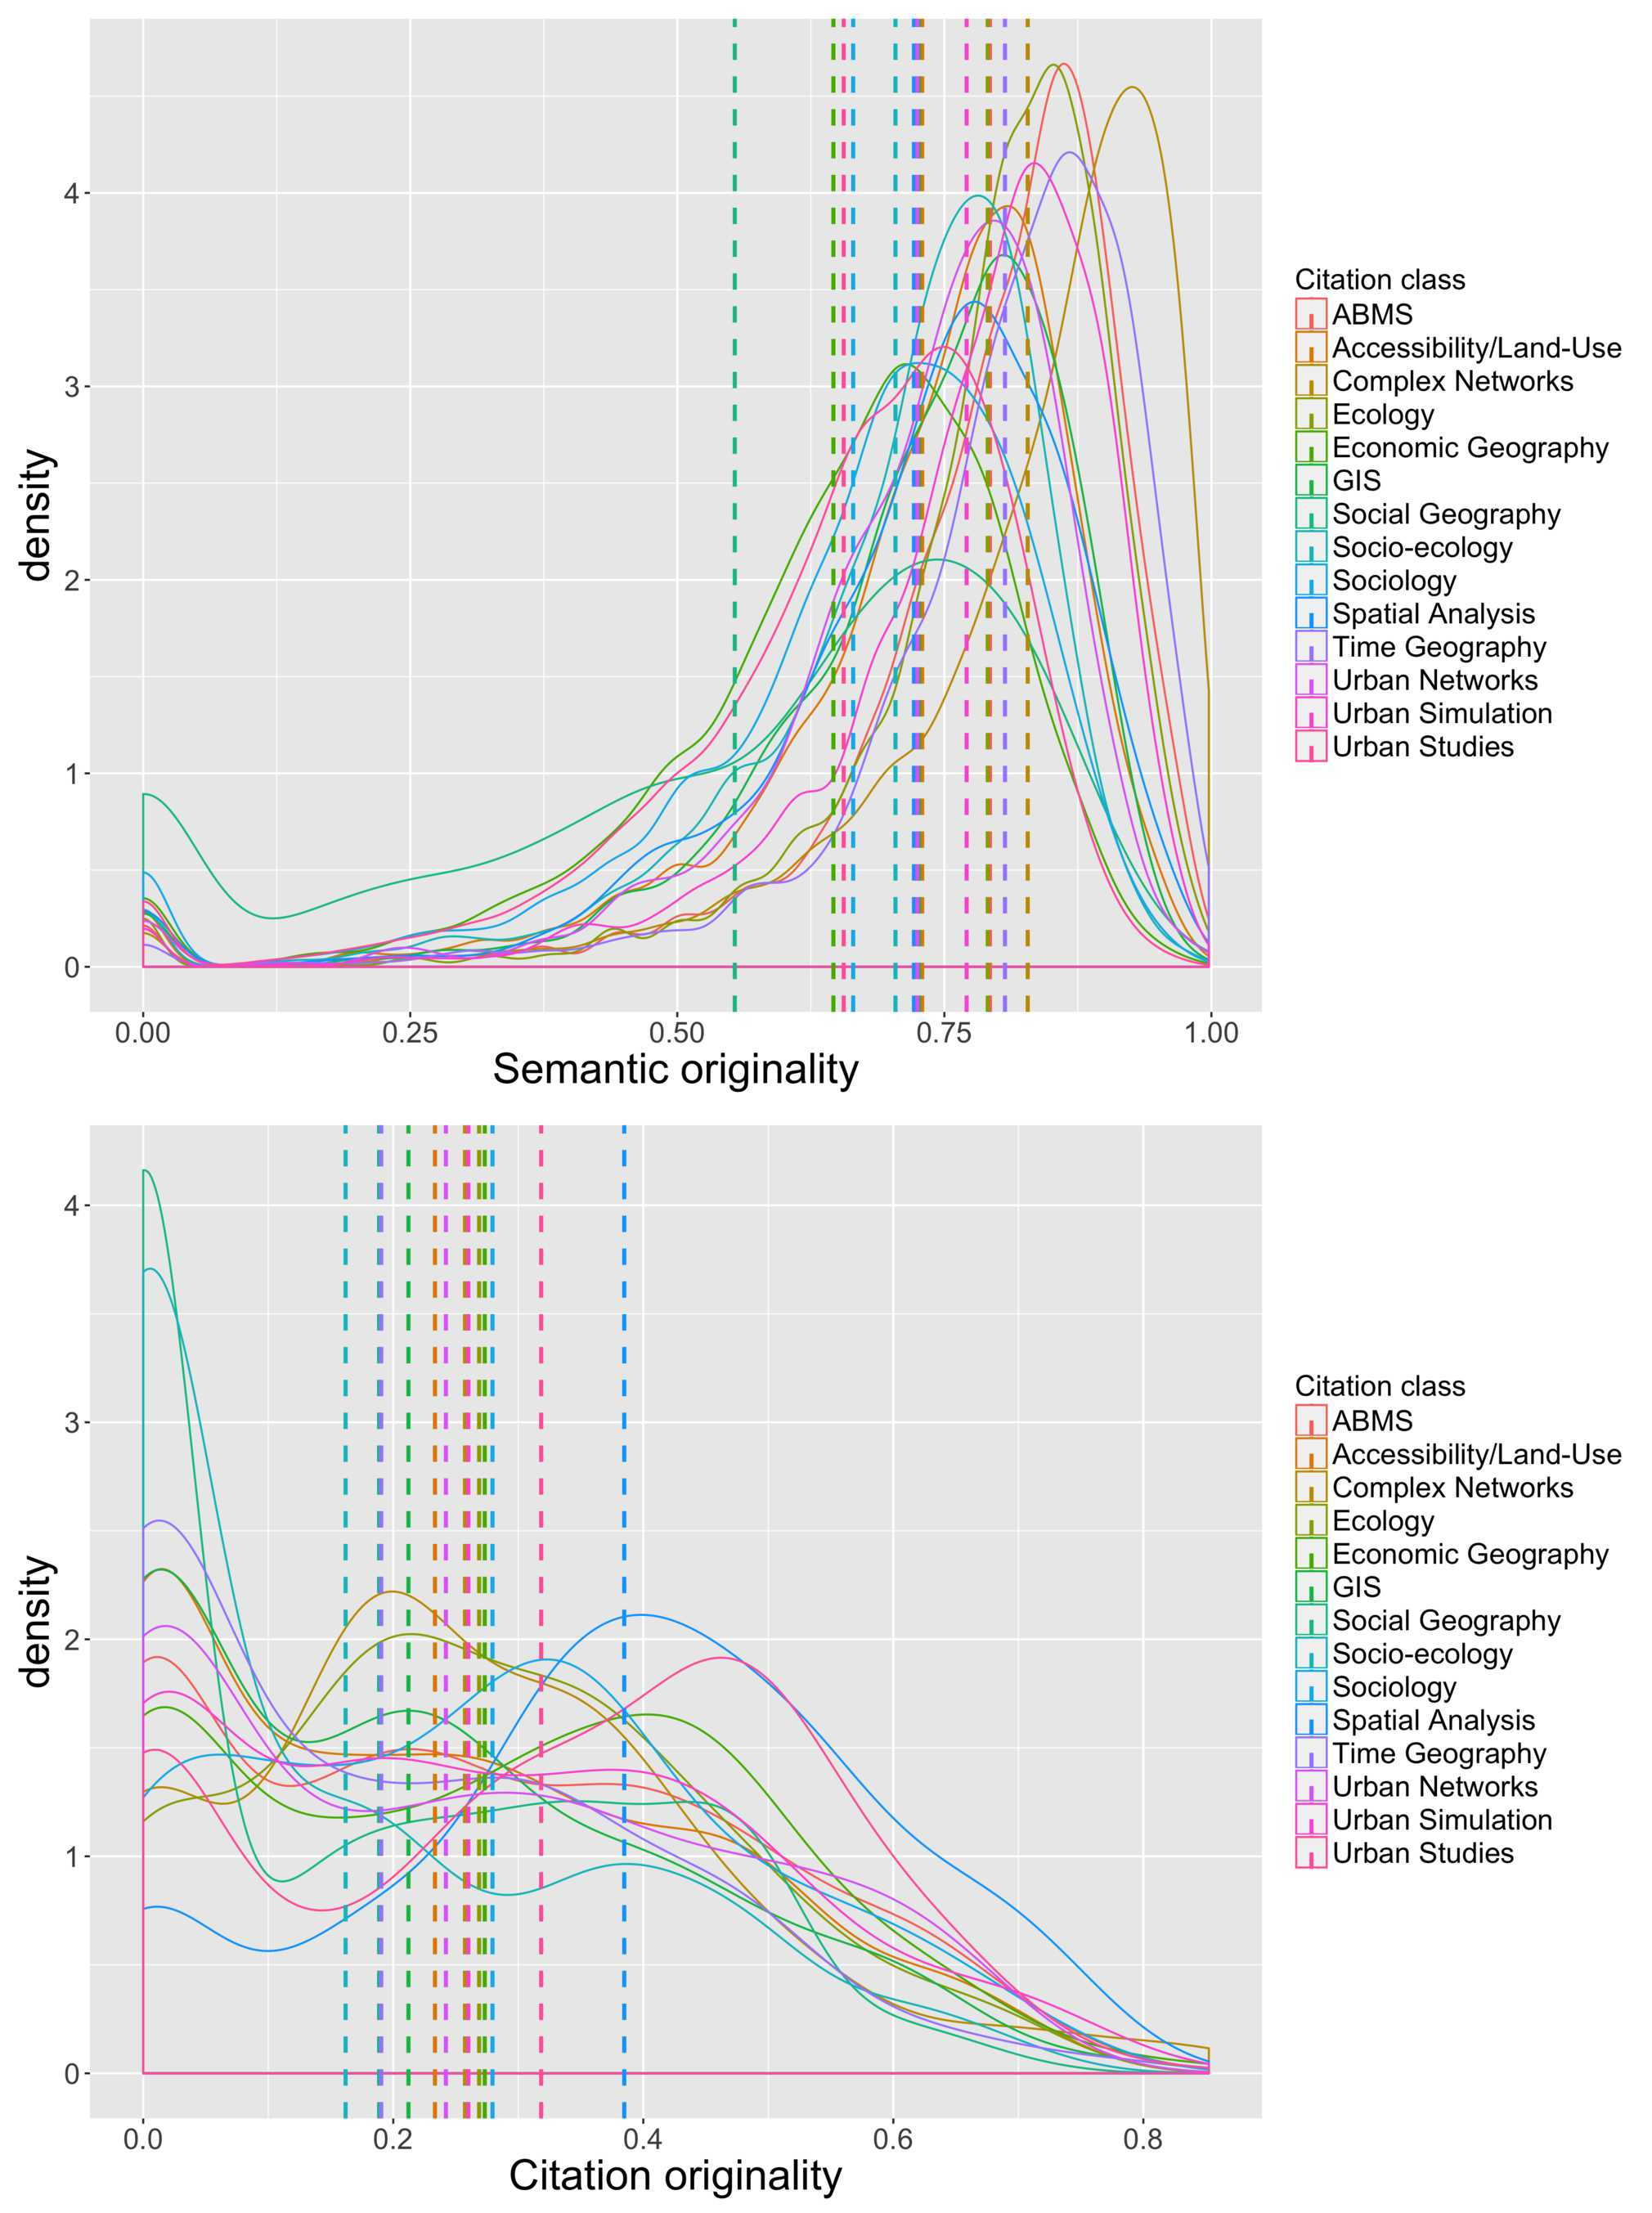
\includegraphics[width=\textwidth]{Figures/Cybergeo/Fig10}
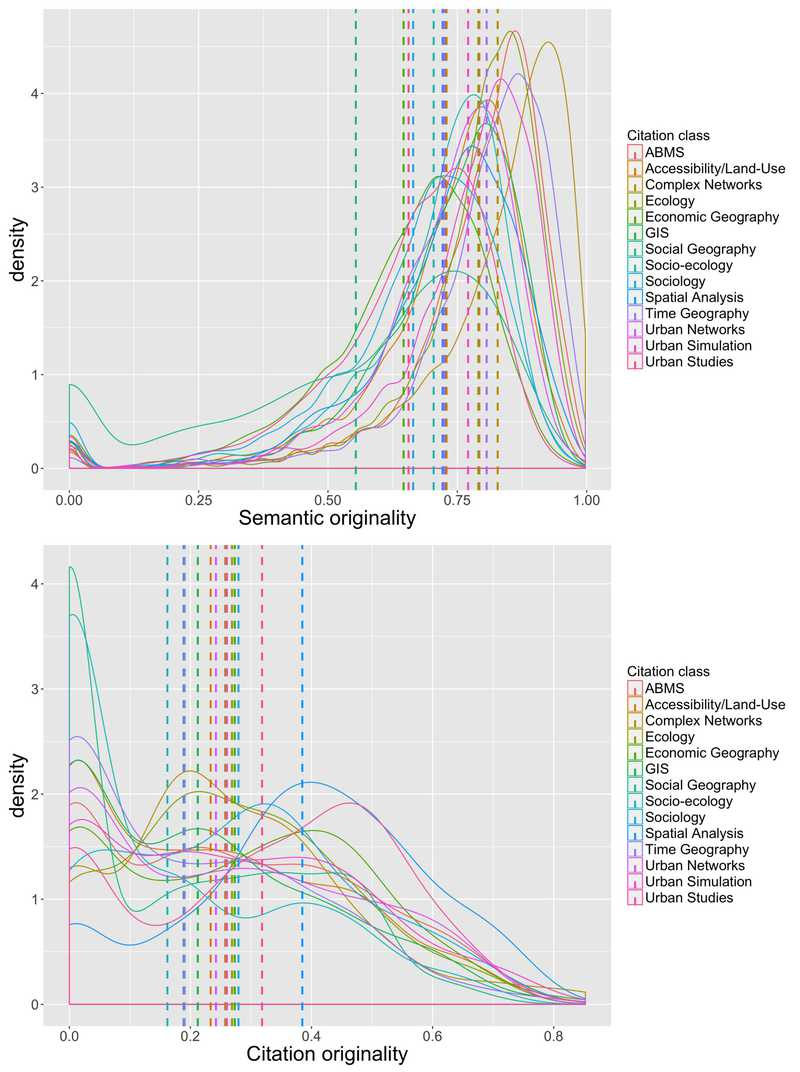
\includegraphics[width=\linewidth]{Figures/Final/B-cybergeo-fig10.jpg}
\caption{\textbf{Statistical distribution of originalities.} We show the smoothed probability densities of originality indexes, by citation class (given by color), for the Semantic originality $o^{(Semantic)}$ (top plot) and for the Citation originality $o^{(Citation)}$ (bottom plot). Dashed lines give the mean for each distribution, with the corresponding color.\label{fig:cybergeo:fig10}}{\textbf{Distribution statistique des originalités.}\label{fig:cybergeo:fig10}}
\end{figure}
%%%%%%%%%%%%%%%%%%


We had up to now a qualitative view on interdisciplinarity patterns, by looking at the relative localisation of communities within the citation and semantic classifications, and the relation between the classifications. We propose now to look at quantitative measures of interdisciplinarity, for each classification.


More precisely, for a given classification $C \in \{ Citation,Semantic\}$ a reference $i$ can be viewed as a probability vector $(p_{ij}^{(C)})_j$ on classes $j$ that give for each class the probability to belong to it. Given this setting, we measure interdisciplinarity of one reference using Herfindhal concentration index~\citep{porter2009science}, that can also be called an originality index. We define originality as
\[
o_i^{(C)} = 1 - \sum_j {p_{ij}^{(C)}}^2
\]

For the semantic classification, probabilities are defined as the proportion of keywords of the abstract within each semantic class. With the deterministic citation classification, each reference has only one class and the originality index is always 0. Therefore in order to be able to compare the two classification, we associate a probability to each citation class for each article as the proportion of citations received from this class. The induced index is original, and measures interdisciplinarity as \emph{how a reference is used} by different disciplines in its lifetime.


We show in Fig.~\ref{fig:cybergeo:fig10} the statistical distribution for both indexes $o^{(Semantic)}$ and $o^{(Citation)}$, stratified by citation class. This allow a direct comparison between the two and also an indirect comparison by the variation of semantic distribution between citation classes. For the distribution of semantic originalities, all citation classes exhibit a similar pattern, that is a peak around large values and a smaller peak at zero. It means that either references are highly specialized and have keywords in one class only, or they use keywords from different classes in a quite even manner (for comparison, an abstract with half keywords in a class and half in an other gives an originality of 0.5). The most original, i.e. the most mixed, citation class, is Complex Networks, with a distribution clearly detached from others, what would confirm their use as a method with a lot of different problems. Social Geography is from far the less original, with a large number of single class references, and an average far lower than other classes, what would mean an increased presence of compartmentalization within the associated disciplines.


In terms of citation originality index, the global picture is fundamentally different, as average originality indexes are all lower than 0.4 and most of distributions show their mode in 0, meaning that most references are only cited by their own citation class. Again, Social Geography is the less original, confirming a similar behavior in terms of citation practice than in terms of research content. The most original classes in average, with a peak in large values, are Spatial Analysis and Urban Simulation: this corresponds to the fact that these class feature quite generic methods that can be applied in several fields and are cited accordingly. Complex Networks do not reach the same level, but however exhibit a peak around 0.2 and no peak in 0, together with Ecology, suggesting disciplines having still significant impact in other disciplines.


To summarize, we show (i) different patterns of interdisciplinarity, depending on disciplines, in terms of scientific content (semantic) and of scientific impact (citation); and (ii) a strong qualitative difference in behavior of originalities between the two classifications, what suggests their complementarity.



%%%%%%%%%%%%%%%%%%
\subsubsection{Correlation between classifications}{Corrélation entre classifications}


In order to strengthen the idea of a complementarity of classifications, that would each capture different dimensions of processes of knowledge production, we finally look at the correlation matrix between classifications. We use this time effective class probabilities for the citation classification, i.e. a vector of zeros expect with a one at the index of the class of the reference. We compute a Pearson correlation coefficient between classes $k$ (in semantic) and $k'$ (in citation) as
\[
\rho_{k,k'} = \frac{Cov \left[ (p^{(Sem)}_{ik})_i , (p^{(Cit)}_{ik'})_i \right]}{\sqrt{\sigma\left[(p^{(Sem)}_{ik})_i\right]\sigma\left[(p^{(Sem)}_{ik})_i\right]}}
\]

\noindent where the covariance is estimated with the unbiased estimator.


The structure of the correlation matrix recalls the conclusions obtained when studying the semantic composition of citation communities, such as GIS being strongly correlated with GIS ($\rho=0.26$), or Sociology with Political Science ($\rho=0.16$). More importantly for our question are summary statistics of the overall matrix. It has a minimum of $-0.16$ (Ecology (citation) against Political Sciences (semantic)), an average of $-0.002$ and a maximum of $0.33$ (Social geography (citation) and Spatial Analysis (semantic)). The ``high'' values are highly skewed, as the first decile is at $-0.06$ and the last at $0.09$, what means that 80\% of coefficient lie within that interval, corresponding to low correlations. In a nutshell, classifications are consistent as highest correlations are observed where one can expect them, but most of classes are uncorrelated, meaning that the classifications are quite orthogonal and therefore complementary.




%summary(as.numeric(rho))
%      Min.    1st Qu.     Median       Mean    3rd Qu.       Max. 
%-0.1631820 -0.0397953 -0.0187894 -0.0003216  0.0089678  0.3262073 

%summary(as.numeric(rho[,2:ncol(rho)]))
%     Min.   1st Qu.    Median      Mean   3rd Qu.      Max. 
% -0.157525 -0.039676 -0.018789 -0.001669  0.008007  0.326207 


% correlation matrix between classifications

%                                                NA Complex Networks      Ecology Social Geography
%health                                 0.084217277      0.015642565 -0.031280002    -0.0304122878
%crime                                 -0.034264269     -0.027466263 -0.030184851    -0.0109058566
%statistical methods                   -0.045196471     -0.009985336  0.134773697    -0.0427562039
%remote sensing                         0.008677423     -0.039616065  0.004274342    -0.0001037131
%political sciences/critical geography -0.163182024     -0.063553835 -0.157524519     0.0103925609
%traffic modeling                       0.135493504     -0.025760072 -0.053805346    -0.0401532076
%microbiology                           0.005013388      0.069833747  0.175721643    -0.0428300111
%cognitive sciences                    -0.057904751      0.021390559 -0.008878000    -0.0183249948
%spatial analysis                      -0.028954136     -0.040284497  0.038681879     0.3262073464
%GIS                                   -0.068226509     -0.025851971 -0.027627123    -0.0355896609
%biogeography                           0.157670367     -0.065793131  0.155044018    -0.0622661875
%environnment/climate                   0.146864511     -0.016857698  0.081698376    -0.0499190937
%economic geography                    -0.036386086     -0.088454740 -0.131327817    -0.0516875579
%physical geography                     0.155877876     -0.050479420  0.044855501    -0.0342161549
%                                         Sociology          GIS Spatial Analysis         ABMS Socio-ecology
%health                                -0.035281096 -0.027390702    -0.0092406664 -0.028471411  -0.039977735
%crime                                 -0.003511700 -0.016330983    -0.0034925253 -0.026372584  -0.016182744
%statistical methods                    0.006204335  0.009875529     0.0006603197  0.016162014  -0.048901119
%remote sensing                        -0.022526140 -0.008140740     0.0161506994  0.051559757   0.009078915
%political sciences/critical geography  0.164538990  0.070441824    -0.0099431496 -0.070547880   0.092456547
%traffic modeling                       0.006759964  0.003892643    -0.0200454337  0.004937954   0.009572245
%microbiology                          -0.010887689 -0.004926871    -0.0256598780  0.032859898  -0.025374219
%cognitive sciences                     0.189133684  0.021302626    -0.0233197884 -0.012683768  -0.039854983
%spatial analysis                      -0.039550918 -0.026571766    -0.0200352507 -0.019253896  -0.036900317
%GIS                                   -0.044445811  0.266230113    -0.0196994093  0.008379501  -0.048098115
%biogeography                          -0.090286092 -0.047362187    -0.0314376536  0.118217762   0.063732285
%environnment/climate                  -0.061530547 -0.043172212    -0.0228268820 -0.010868666   0.042866717
%economic geography                    -0.007205760 -0.080607481     0.1107474038 -0.087310233  -0.080743040
%physical geography                    -0.077603719 -0.024403758    -0.0309332281 -0.007944706   0.177918682
%                                      Urban Networks Urban Simulation Urban Studies Economic Geography
%health                                   0.227985960      0.003101104  -0.011951445       -0.029092421
%crime                                   -0.007323995      0.151779291   0.037625633        0.007882492
%statistical methods                      0.002304641      0.074944283  -0.047068353       -0.019986633
%remote sensing                           0.011034168     -0.007373975   0.009064606       -0.008777581
%political sciences/critical geography    0.024982340     -0.129188848   0.250087262        0.123687818
%traffic modeling                        -0.026107672     -0.016873541  -0.020788824       -0.056640509
%microbiology                            -0.031639788     -0.015875901  -0.048817564       -0.039139437
%cognitive sciences                      -0.024141333      0.006168384  -0.017845169       -0.051689224
%spatial analysis                        -0.022931057      0.004936436  -0.048686678       -0.027250467
%GIS                                     -0.031369284      0.107217335  -0.059539768       -0.055057115
%biogeography                            -0.038744405     -0.019857075  -0.093015237       -0.081157234
%environnment/climate                    -0.003931271     -0.009427780  -0.061113194       -0.052661932
%economic geography                       0.035747109      0.070533726   0.036039127        0.154483917
%physical geography                      -0.013960728     -0.003533876  -0.058702622       -0.064289131
%                                      Accessibility/Land-Use Time Geography
%health                                          -0.020422023   -0.026027683
%crime                                           -0.009526164   -0.019419266
%statistical methods                             -0.008130459   -0.008458811
%remote sensing                                  -0.009152899   -0.023371493
%political sciences/critical geography           -0.073794569   -0.017737603
%traffic modeling                                 0.035398096   -0.020400327
%microbiology                                    -0.055066210   -0.003858738
%cognitive sciences                              -0.049222763    0.141081799
%spatial analysis                                 0.007710532   -0.009041103
%GIS                                             -0.033615280    0.237580646
%biogeography                                    -0.029578349   -0.062363162
%environnment/climate                             0.012457860   -0.055488257
%economic geography                               0.213283602   -0.087410630
%physical geography                              -0.069686740   -0.037465822
%








%%%%%%%%%%%%%%%%%%
\subsection{Discussion}{Discussion}
%%%%%%%%%%%%%%%%%%

We have this way shown the complementarity of classifications in the qualitative patterns they unveil, but also quantitatively in terms of interdisciplinarity measures and quantitatively in terms of correlations. Our work can be extended regarding several aspects, of which we give some suggestions below.


\subsubsection{Further Developments}{Développements}

A first development consists in the comparison of journals. The starting point for construction of the scientific environment, the journal \textit{Cybergeo}, was the entry point but not the subject of our study. A development more focused on journals, trying for example to answer comparative issues, or to classify journals according to their effective level of interdisciplinarity regarding different dimensions, would be potentially interesting. The collection of precise data on the origin of references is however a first step that need to be solved first.


The performance of the semantic classification was also not quantified here. A further validation of the relevance of using complementary information contained in both classifications could be done by the analysis of modularities within the citation network, as done in~\cite{bergeaud2017classifying}. This would however require a baseline classification to compare with, which is not available in the type of data we use. Open repository such as arXiv (for physics mainly) or Repec (for Economics) provide API to access metadata including abstracts, and could be starting points for such targeted case studies.




\subsubsection{Applications}{Applications}


A first potential application of our methodology relies on the facts that both classifications unveils thematic domains (objects of study), classical disciplines, methodological communities. These different types of communities can indeed be understood as different \emph{Knowledge Domains}. \cite{raimbault2017applied} postulates co-evolving Knowledge Domains in every process of scientific knowledge production, that are Theoretical, Empirical, Modeling, Methodology, Tools and Data domains. Most of them are necessary for any process, and investigations within one conditions the advances in others. A refinement of classifications, associated with supervised classification to associate knowledge domains to some communities (potentially using full texts to have more precise information on the proportion of each knowledge domains involved in each), would allow to quantify relations between domains. Furthermore, using temporal data with the date of publications, would yield an effective quantification of the \emph{co-evolution} of domains in the sense of patterns of temporal correlations (e.g. Granger causality).

An other interesting direction is the application of our classifications to the quantification of spatial diffusion of knowledge, as \cite{maisonobe2013diffusion} does for the diffusion of a specific question in genetics. It is not clear if different dimensions of knowledge diffuse the same way: for example citation practices can be correlated to social networks and thus exhibit different patterns than effective research contents. Therefore, our work would allow to study such questions from complementary point of views.


Finally, we believe the tool we developed can contribute to an increased empowerment of authors and to the development of open science practices. Among the various visions of Open Science~\citep{fecher2014open}, the opening of data is always an important aspect, together with a development of reflexivity in all disciplines, beyond the sole Social Sciences to which it is classically associated. The first point is dealt with by our open tools for dataset construction, whereas the second is implied by the new knowledge of the different dimensions of the scientific environment we studied.








%%%%%%%%%%%%%%%%%%
\subsection{Conclusion}{Conclusion}
%%%%%%%%%%%%%%%%%%


We have introduced a multi-dimensional approach to the understanding of interdisciplinarity, based on citation network and semantic network analysis. Starting from a generalist journal in Geography, we construct a large corpus of the citation neighborhood, from which we extract relevant keywords to elaborate a semantic classification. We then show qualitatively and quantitatively the complementarity of classifications. The methodology and associated tools are open and can be reused in similar studies for which data is difficult to access or poorly referenced in classical databases.




%%%%%%%%%%%%%%%%%%%%%
%%%%%%%%%%%%%%%%%%%%%

\subsection*{acknowledgements}{Remerciements}
The author would like to thank the editorial board of Cybergeo, and more particularly Denise Pumain and Christine Kosmopoulos, for having offered the opportunity to work on that subject and provided the production database of the journal. 





